\graphicspath{{./images/}}      
\def\CHAPTERONE{./chapters/Chapter-1} 

\chapter{Experimente}
\label{chap:experiments}
%	\input{\CHAPTERONE /motivation}

Im folgenden Kapitel werden zuerst die für die Arbeit erstellten Datensätze erläutert. Danach werden die Experimente beschrieben, die im Rahmen dieser Arbeit durchgeführt wurden, um die Objektklassifikation mit fotorealistischen Bildern zu evaluieren. \newline
In einem ersten Experiment werden \glspl{klassifikator} trainiert und mit den Unreal-Bildern getestet. Danach wird ein \gls{mln} mit den Unreal-Bildern trainiert und getestet. Zur Evaluation wird 10-fache Kreuzvalidierung durchgeführt. Danach wird ein \gls{mln} mit den Unreal-Bildern trainiert und mit realen Bildern getestet. Zum Abschluss wird ein Teil der realen Bilder mit in die Trainingsdaten aufgenommen und mit dem Rest getestet. Jedes Experiment wird zweimal durchgeführt: einmal mit den Objektklassen als \gls{gt} und einmal mit den Instanznamen der Objekte. Eine Übersicht  der Ergebnisse kann auf Seite \pageref{tab:classification_all} in Tabelle \ref{tab:classification_all} gefunden werden. Dabei werden auch die Ergebnisse aus \cite{pr2looking} mit angegeben. Darin wurde ein \gls{mln} mit realen Bildern trainiert und getestet und die Ergebnisse dienen als Vergleichswerte der in dieser Arbeit durchgeführten Experimente.

\section{Erklärung und Analyse der Datensätze}

In diesem Abschnitt wird beschrieben, wie sich Szenen der Unreal-Bilder zusammensetzen und die Häufigkeit des Auftretens der einzelnen Klassen und Instanzen analysiert. Da das Ziel ist, ein \gls{mln} mit den Unreal-Bildern zu trainieren und mit diesem echte Bilder zu klassifizieren, wurde auch ein Satz echter Bilder aufgenommen. Dieser wird hier auch erläutert.

\subsection{Unreal-Bilder}  
Für die Experimente wurden mit dem in Kapitel \ref{sec:takingpics} vorgestellten Verfahren 114 Szenen erstellt und von ihnen fünf Bilder aufgenommen (Beispielszene auf Seite \pageref{fig:exampleScene}, Abbildung \ref{fig:exampleScene}). Jede Szene enthält zwischen 2 und 5 Objekte. Die Objekte haben dabei ausreichend Abstand zueinander, um eine eindeutige Identifizierung zuzulassen. Jedes Objekt ist mindestens einem der folgenden Szenarios zugeordnet: \textit{breakfast}, \textit{cooking} oder \textit{fridge}. Die Zuordnung ist in Tabelle \ref{tab:objects} einzusehen. Eine Szene enthält nur Objekte eines Szenarios. Dies ist echten Bedingungen nachempfunden, denn in der Regel finden sich im Kühlschrank keine Gabeln, Milch allerdings schon, die wiederum auch auf einem Frühstückstisch zu finden sein kann. Es wurden jeweils 50 \textit{breakfast} und \textit{cooking} Szenen sowie 14 \textit{fridge} Szenen erstellt. Insgesamt stehen so \textbf{570 Unreal-Bilder} zur Verfügung. \par

In Abbildung \ref{fig:Unreal-Images_analysis} ist die Verteilung der Objekte in den gesamten Unreal-Bildern zu sehen. Ein Großteil der Objektinstanzen kommt in einer ähnlichen Anzahl in den Bildern vor. Die mehreren Szenarien zugeordneten Objekte, wie der \textit{AlbiHimbeerJuice} dem \textit{breakfast} und \textit{cooking}, jedoch bis zu doppelt so häufig. Dies ist durch die Art der Erstellung der Unreal-Bilder zu erklären: Es wurde versucht, pro Szenario eine gleichmäßige Verteilung zu erreichen. \newline
Die ungleiche Verteilung der Objektklassen ist bedingt durch die unterschiedliche Anzahl an Objektinstanzen pro Klasse. Es gibt beispielsweise nur ein Objekt, dass der \textit{Coffee} Klasse angehört, jedoch vier Objekte, die der \textit{Bowl} Klasse angehören. \newline
Es wird dementsprechend von einem ungleich verteilten Datensatz ausgegangen. Bei der Berechnung der Fehlergrößen \gls{precision}, \gls{recall} und \gls{f1score} der Klassifikation des gesamten Datensatzes wird deshalb der gewichtete Durchschnitt der Fehlergrößen pro Instanz/Klasse verwendet. Das Gewicht wird dabei durch die Anzahl der richtigen Einordnungen beschrieben. \par

\begin{figure}
\centering
	\begin{subfigure}[b]{0.4\textwidth}
	\centering
		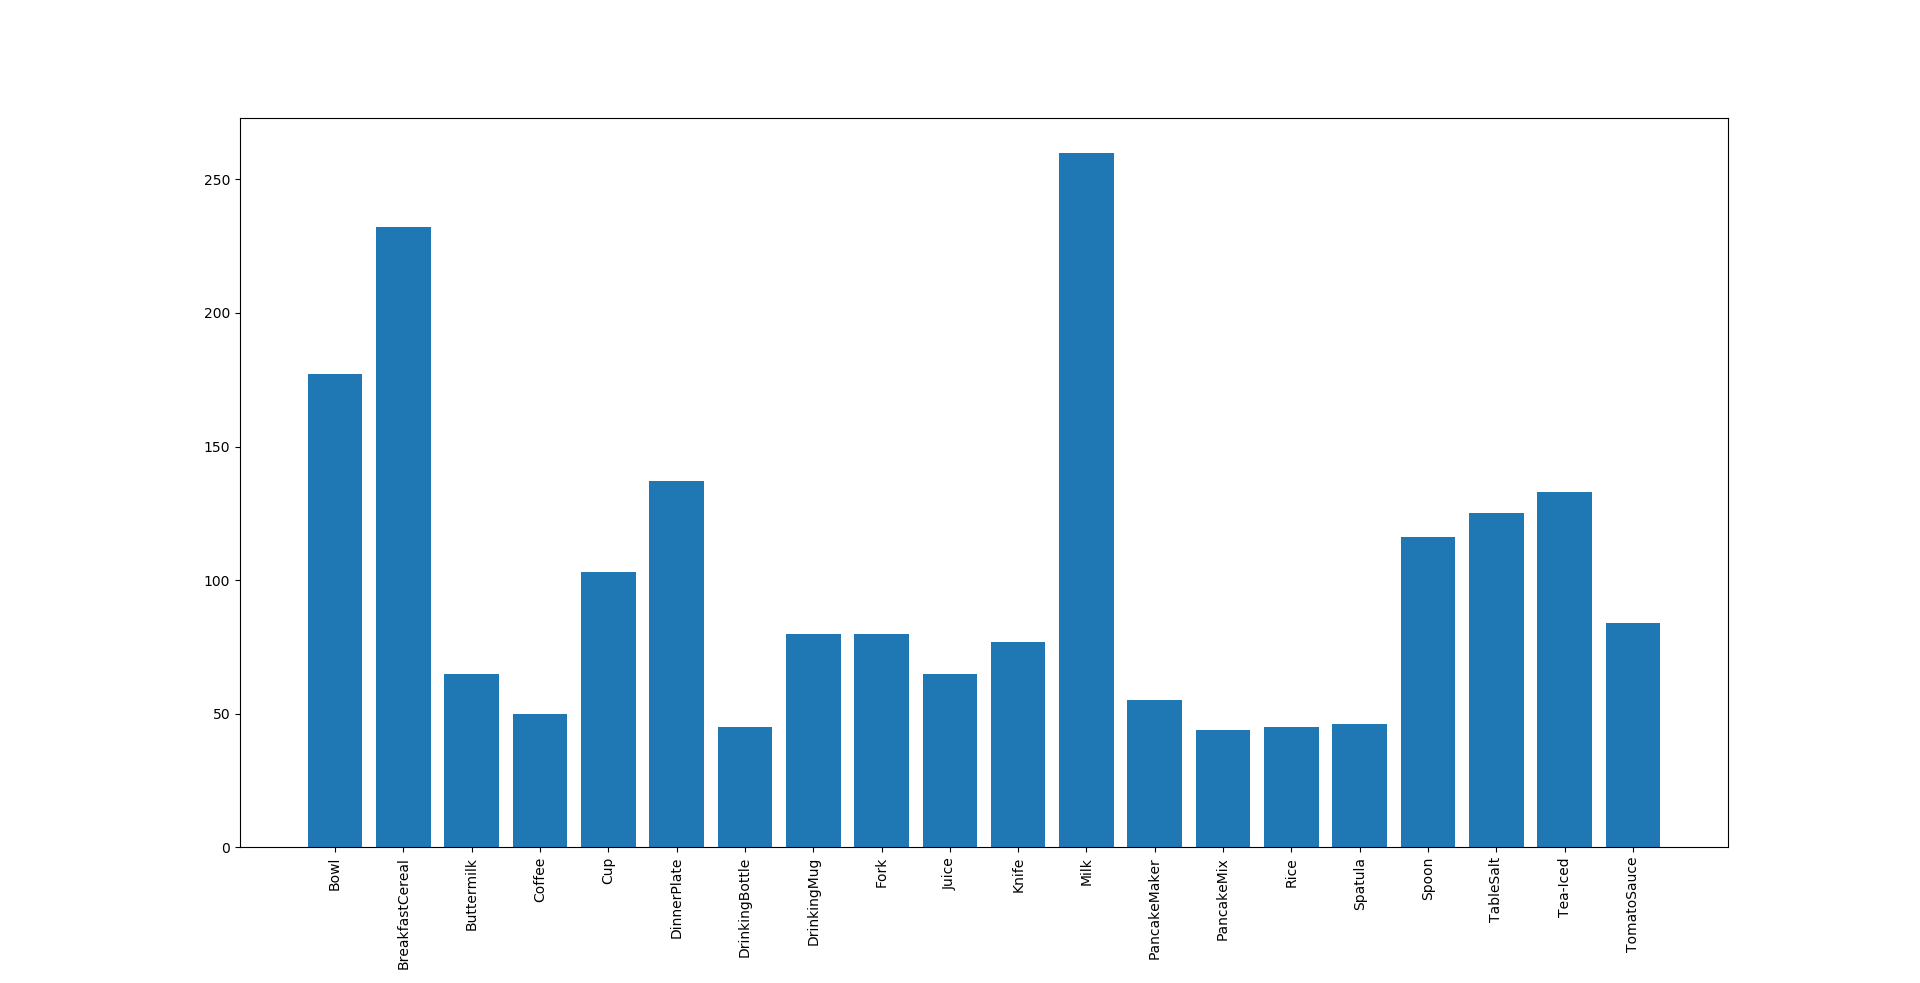
\includegraphics[scale=.4]{img/chapter6/UnrealGTClass_analysis.png}
	\end{subfigure}
	\begin{subfigure}[b]{0.58\textwidth}
	\centering
		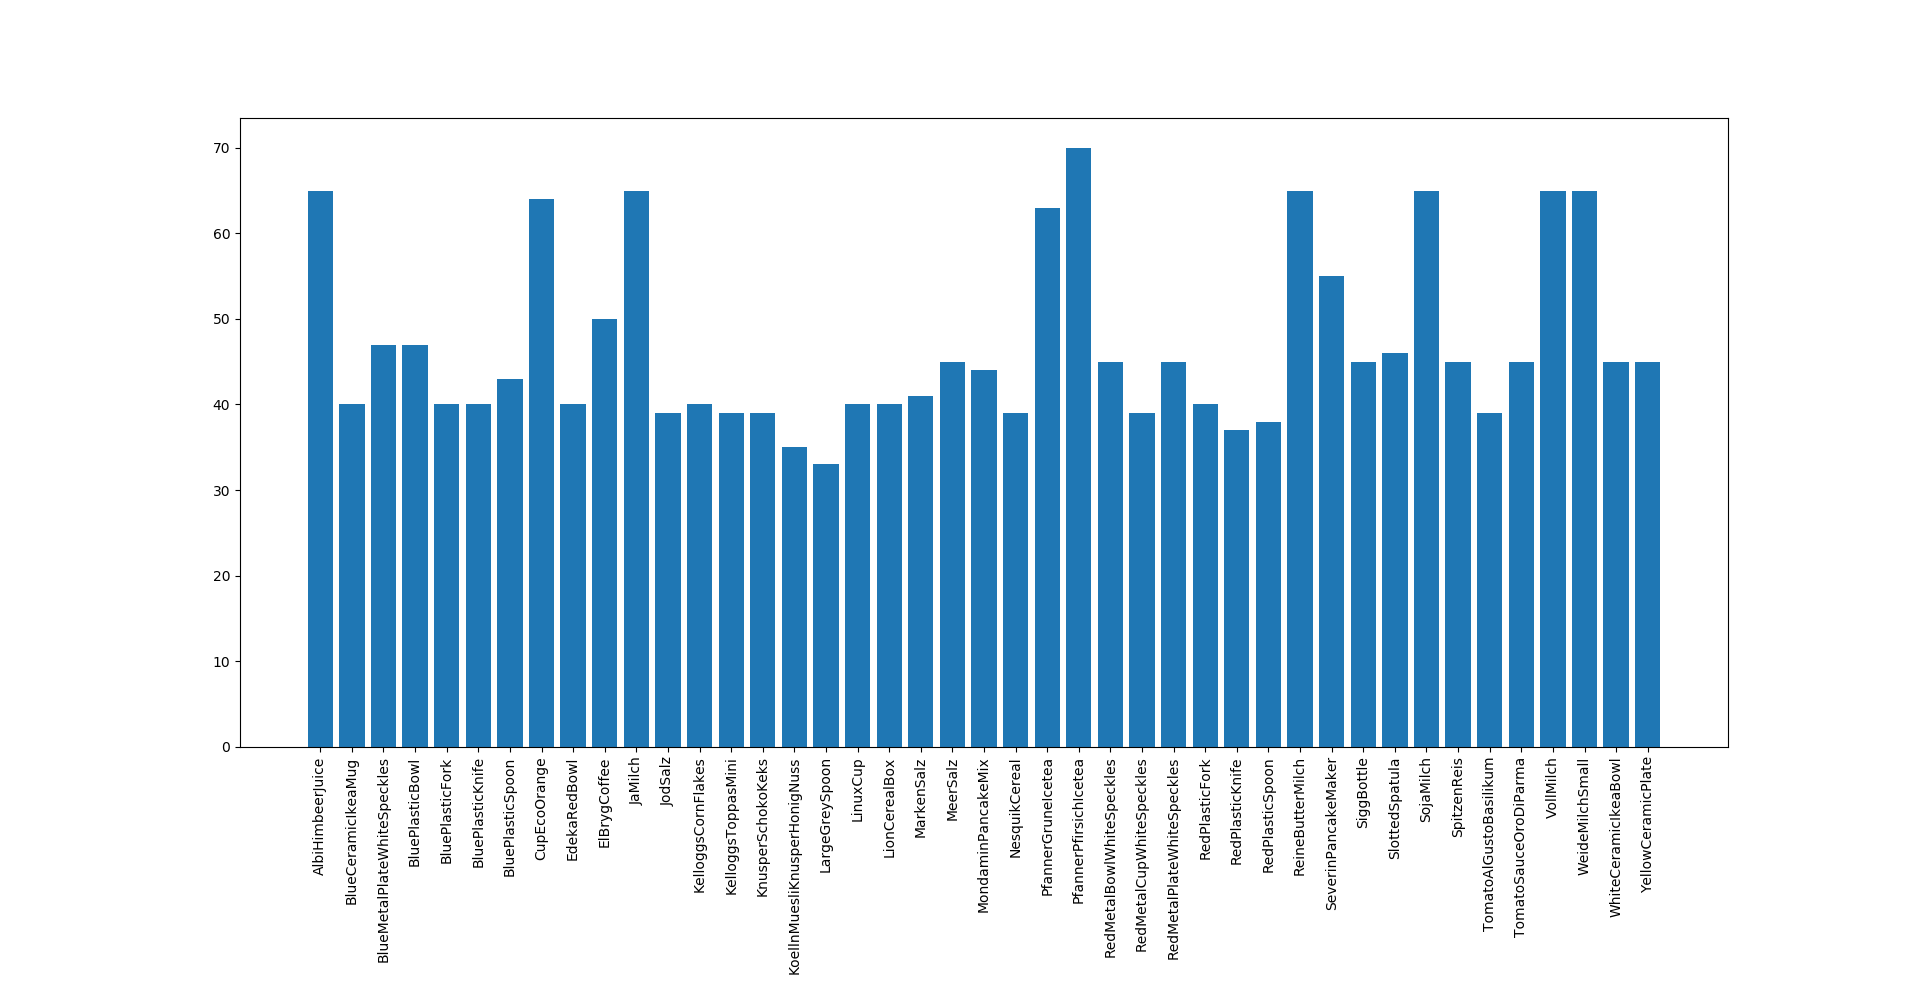
\includegraphics[scale=.4]{img/chapter6/UnrealGTInstance_analysis.png}	
	\end{subfigure}
\caption[Verteilung der Objekte in den Unreal-Bildern]{Verteilung der Objektklassen und Instanzen in den gesamten Unreal-Bildern.}
\label{fig:Unreal-Images_analysis}
\end{figure}

\subsection{Reale Bilder}
Mit dem PR2-Roboter des \gls{iai} wurden Bilder in der realen Küchenumgebung aufgenommen. Die verwendeten Objekte sind dabei die Vorlagen der Assets, also die ursprünglich eingescannten Objekte. Unglücklicherweise stand zu dem Zeitpunkt der Aufnahme der \textit{LinuxCup} und die \textit{YellowPlate} nicht mehr zur Verfügung. Für die \textit{YellowPlate} wurde stattdessen ein weißer Teller als Ersatzobjekt verwendet. Es wurden wieder 114 Szenen mit der gleichen Szenarien-Verteilung und den gleichen Bedingungen erstellt. Auf Grund des erhöhten Aufwandes bei der Aufnahme der Szenen wurden von jeder Szene nur drei Bilder aufgenommen, womit insgesamt \textbf{342 reale Bilder} zur Verfügung stehen. Im Gegensatz zu den Unreal-Bildern sind die Blickwinkel nicht für jede Szene exakt die gleichen, da der Roboter bei der Aufnahme manuell bewegt werden muss (eine Szene ist in Abbildung \ref{fig:exampleSceneReal} zu sehen). \par

\begin{figure}
\centering
	\begin{subfigure}[b]{0.3\textwidth}
		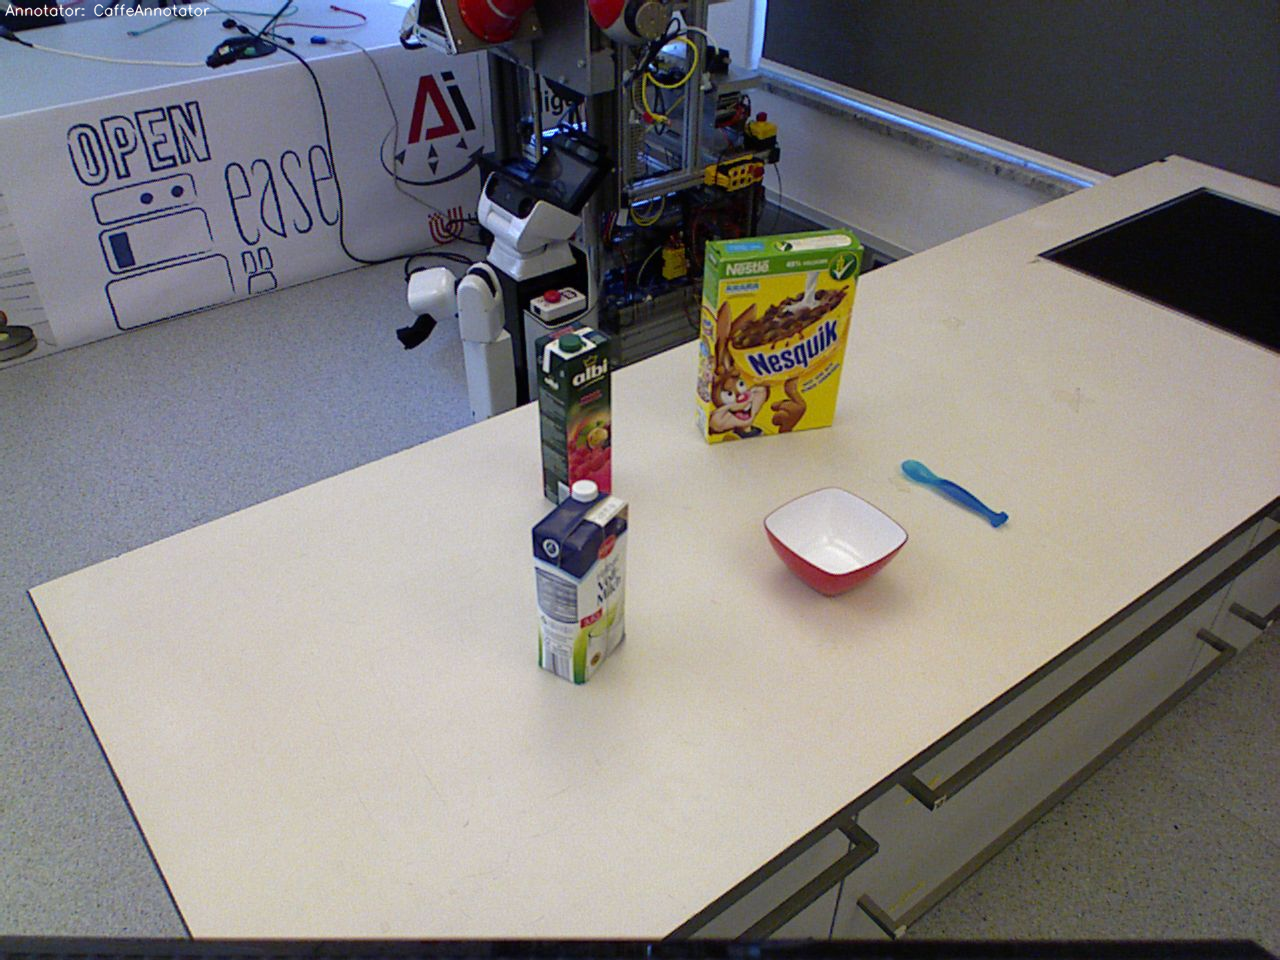
\includegraphics[scale=.1]{img/chapter6/real1}
	\end{subfigure}
	\quad
	\begin{subfigure}[b]{0.3\textwidth}
		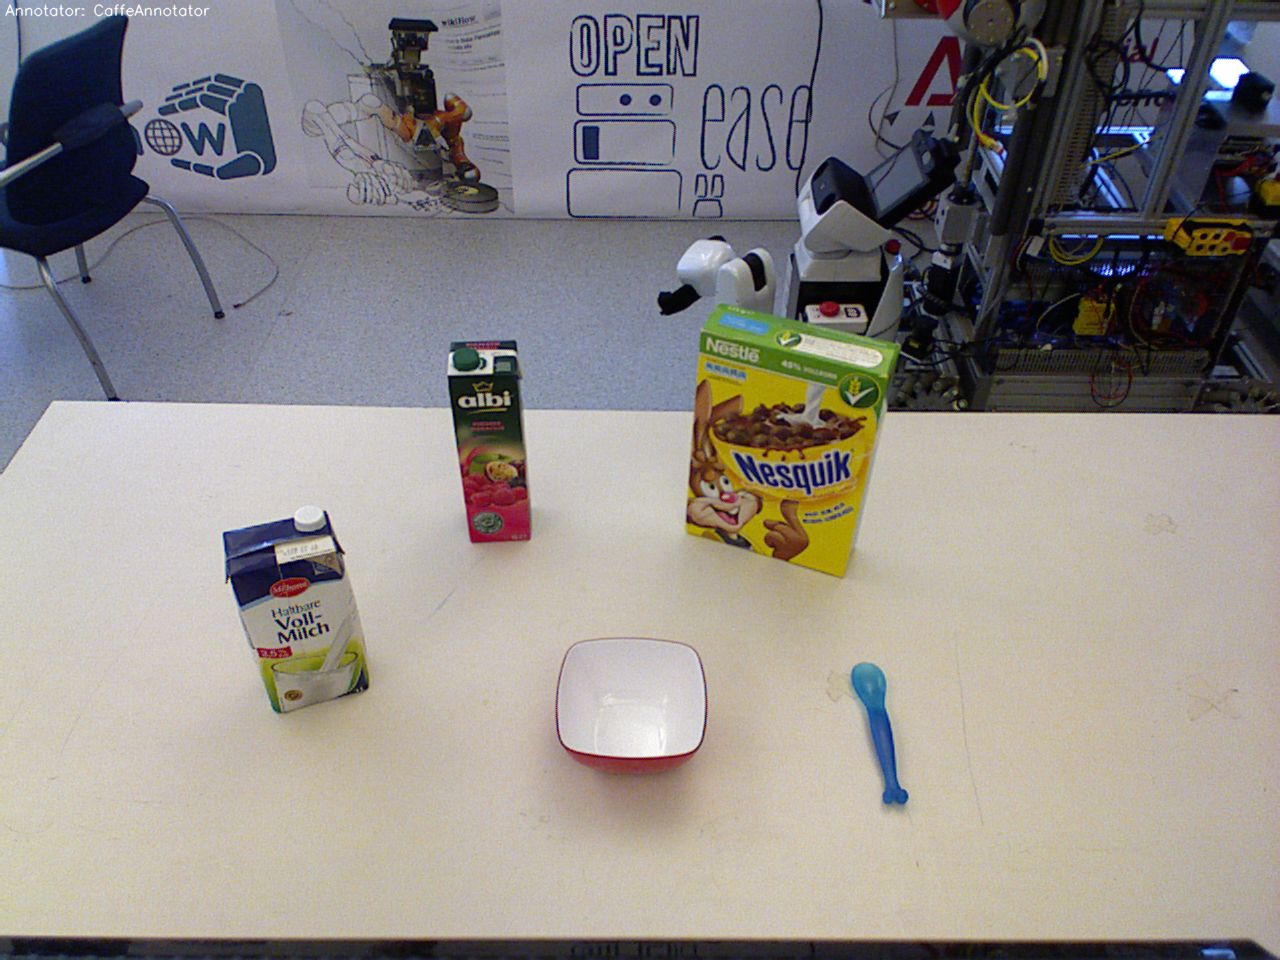
\includegraphics[scale=.1]{img/chapter6/real2}	
	\end{subfigure}
	\quad
	\begin{subfigure}[b]{0.3\textwidth}
		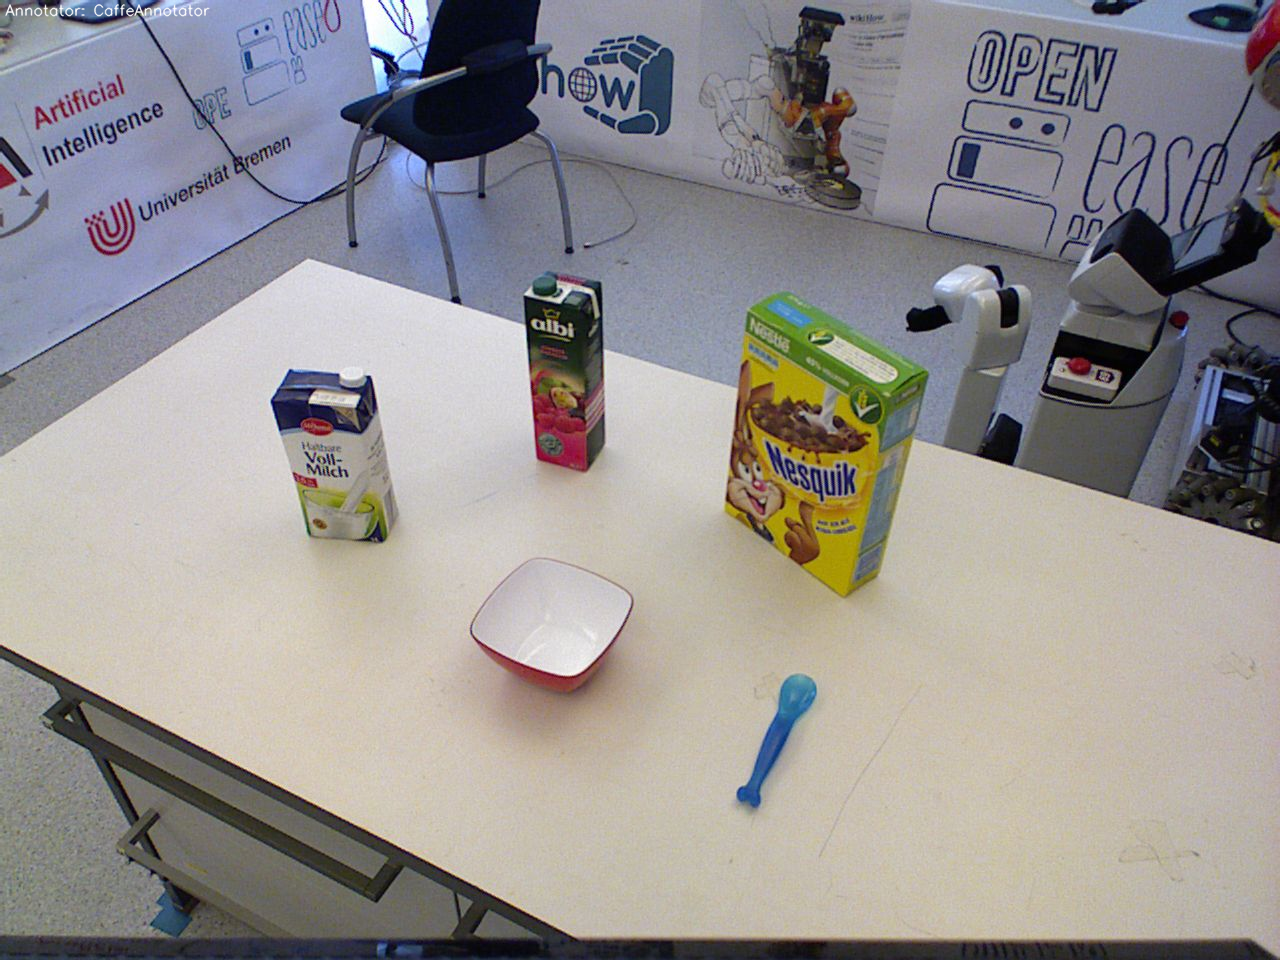
\includegraphics[scale=.1]{img/chapter6/real3}	
	\end{subfigure}
\caption[Reale Bilder einer Szene]{Ein Bildersatz der realen Szenen.}
\label{fig:exampleSceneReal}
\end{figure}

\begin{figure}
\centering
	\begin{subfigure}[b]{0.4\textwidth}
	\centering
		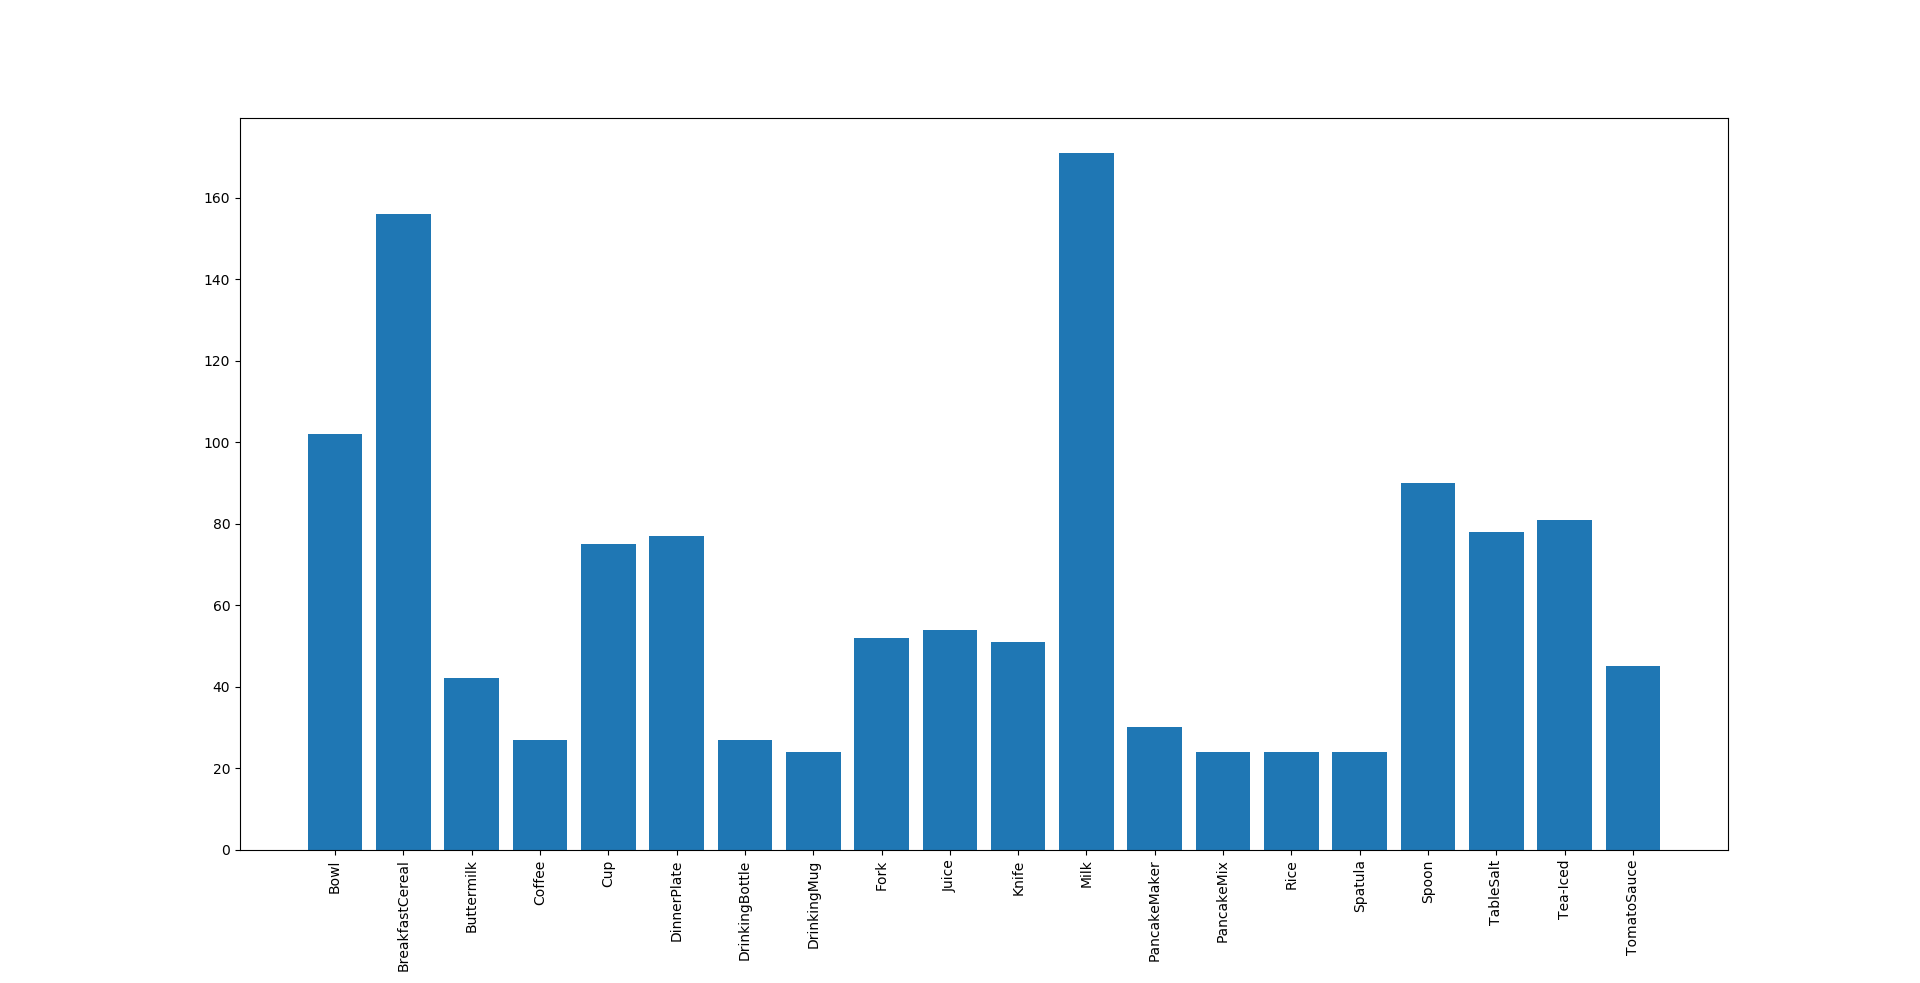
\includegraphics[scale=.4]{img/chapter6/RealGTClass_analysis.png}
	\end{subfigure}
	\begin{subfigure}[b]{0.58\textwidth}
	\centering
		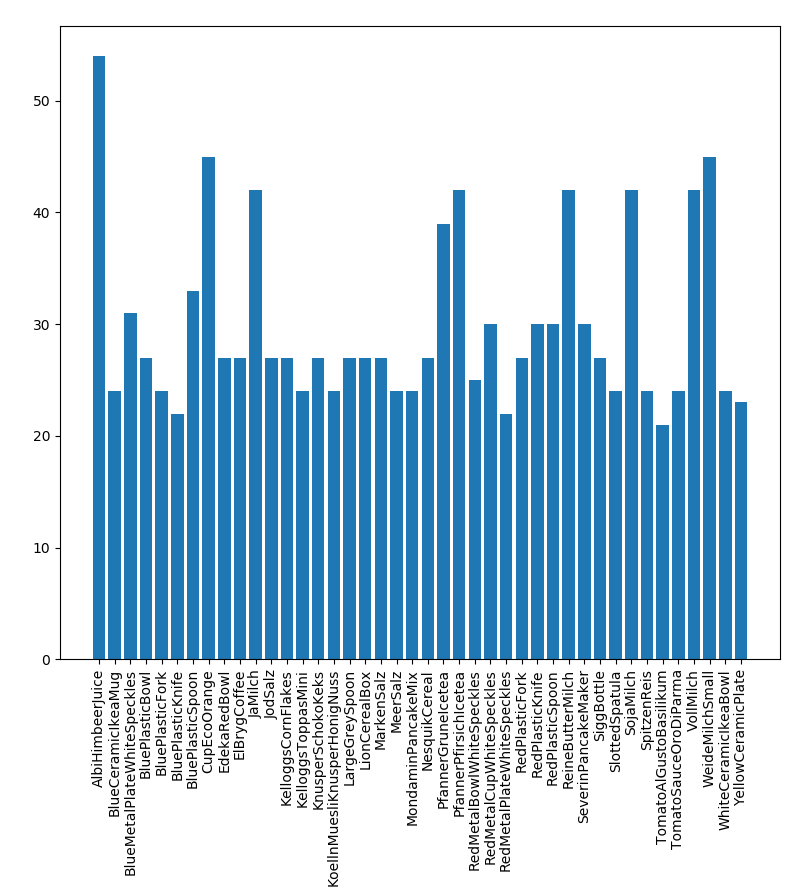
\includegraphics[scale=.4]{img/chapter6/RealGTInstance_analysis.png}	
	\end{subfigure}
\caption[Verteilung der Objekte in den Unreal-Bildern]{Verteilung der Objektklassen und Instanzen in den gesamten Unreal-Bildern.}
\label{fig:Real-Images_analysis}
\end{figure}

Die Verteilung der Objektklassen und Instanzen in den realen Bildern, zu sehen in Abbildung \ref{fig:Real-Images_analysis}, zeigt die gleichen Eigenschaften, wie die Verteilung der Unreal-Bilder. Es wird auch hier von einem ungleich verteilten Datensatz ausgegangen. 


\section{Klassifizierung mit Klassifikatoren}
\label{sec:classificationExperiment}
Die zuvor erstellten Unreal-Bilder wurden in ersten Experimenten über \gls{feature} klassifiziert. Dazu wurde ein Annotator aus dem \robosherlock-Paket \textit{rs\_addons} als \gls{klassifikator} mit echten Bildern der verwendeten Objekte trainiert. Mehr zu dem Paket und den \glspl{klassifikator} ist in Kapitel \ref{sec:classifiers} auf Seite \pageref{sec:classifiers} zu finden. \par

Als \glspl{klassifikator} wurden der \texttt{RFAnnotator} und der \texttt{SVMAnnotator} verwendet, die jeweils auf einer \gls{rf} oder \gls{svm} Implementierung basieren. Die Objekte sollten in zwei Versuchsreihen entweder den Objektklassen oder den Instanznamen zugeordnet werden. Vor dem Training der \glspl{klassifikator} wurden die Bilder der echten Objekte den Klassen/Instanzen zugeordnet. Da es sich um Annotatoren für \robosherlock handelt, wurde eine \gls{ae} mit einigen \textit{hyotheses generators}, dem \texttt{CaffeAnnotator} zum Extrahieren der Merkmale (siehe Kap. \ref{sec:caffeAnno}, S.\pageref{sec:caffeAnno}), dem\linebreak \texttt{UnrealGTAnnotator} zum extrahieren der \gls{gt} und dem jeweiligen \gls{klassifikator} erstellt. Um die Ergebnisse später verarbeiten zu können, wurden sie mit dem \texttt{MLNInferencer} (siehe Kap. \ref{sec:mlnInferencer}, S. \pageref{sec:mlnInferencer}) als logische Prädikate ausgegeben. Die so erhaltene Klassifizierung wird für jedes Objekt mit der \gls{gt} verglichen, um so die Klassifikationsrate des \gls{klassifikator}s zu ermitteln.


\subsection{Objektklassen}
Die Ergebnisse des \texttt{RFAnnotators} sind in Abbildung \ref{fig:RFClassifierGTClass_confMatrix} und Tabelle \ref{tab:RFClassifierGTClass_metrics} abgebildet. Während nahezu alle Objekte eine \gls{accuracy} über 90\% aufweisen, zeigen \gls{precision}, \gls{recall} und \gls{f1score}, dass der \texttt{RFAnnotator} große Schwierigkeiten hat, visuell ähnliche Objekte auseinander zu halten. Besonders häufig werden Objekte fälschlicherweise als \textit{Milk} und \textit{TableSalt} eingeordnet. Dies ist auf die box-artige Form und die Farbähnlichkeit vieler Objekte der beiden Klassen zurückzuführen, welche insgesamt auch in größerer Zahl in den Daten vorkommen als andere Objektklassen. Des weiteren hat der \gls{klassifikator} Schwierigkeiten, das Geschirr auseinander zu halten, was auf die Größe dessen zurückzuführen ist. Besonders schlecht schneidet der \textit{Spatula} ab, der nicht einmal korrekt erkannt wurde. Mit einem \gls{f1score} über 80\% schneiden die Objektklassen \textit{Buttermilk}, \textit{Coffee}, \textit{Cup} und \textit{PancakeMix} am besten ab. Diese Klassen unterscheiden sich in Form (\textit{Buttermilk}, \textit{PancakeMix}) und Farbe (\textit{Coffee}, \textit{Cup}) stark von den anderen Objekten.  \par


\begin{figure}
\centering
	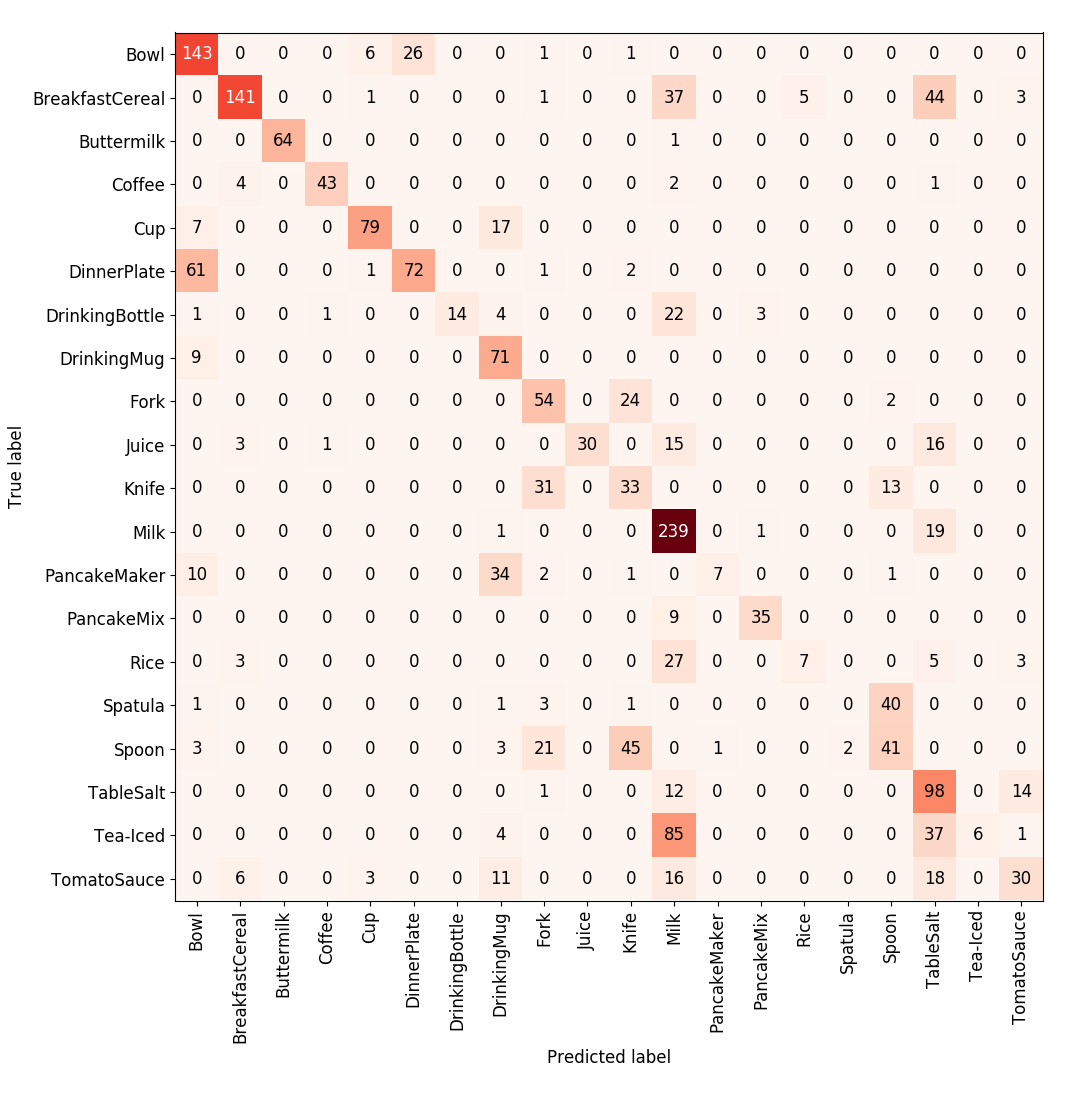
\includegraphics[scale=.315]{img/chapter6/RFClassifierGTClass.png}
\caption[Konfusionsmatrix der Klassifizierung der Objektklassen durch den RFAnnotator]{Die Konfusionsmatrix für die Objektklassen Klassifikation der Unreal-Bilder durch den mit echten Bildern trainierten \texttt{RFAnnotator}.}
\label{fig:RFClassifierGTClass_confMatrix}
\end{figure}

\begin{table}
\centering
\small
\rowcolors{1}{}{lightgray}
\begin{tabularx}{\textwidth}{Xllll}
\textbf{Objekt}	& \textbf{\gls{accuracy}} & \textbf{\gls{precision}}	& \textbf{\gls{recall}}	& \textbf{\gls{f1score}} \\ \hline
Bowl & 0.91 & 0.61 & 0.81 & 0.69 \\  
BreakfastCereal & 0.92 & 0.9 & 0.61 & 0.72 \\  
Buttermilk & 1.0 & 1.0 & 0.98 & 0.99 \\  
Coffee & 0.99 & 0.96 & 0.86 & 0.91 \\  
Cup & 0.97 & 0.88 & 0.77 & 0.82 \\  
DinnerPlate & 0.93 & 0.73 & 0.53 & 0.61 \\  
DrinkingBottle & 0.97 & 1.0 & 0.31 & 0.47 \\  
DrinkingMug & 0.93 & 0.49 & 0.89 & 0.63 \\  
Fork & 0.93 & 0.47 & 0.68 & 0.55 \\  
Juice & 0.97 & 1.0 & 0.46 & 0.63 \\  
Knife & 0.91 & 0.31 & 0.43 & 0.36 \\  
Milk & 0.83 & 0.51 & 0.92 & 0.66 \\  
PancakeMaker & 0.96 & 0.88 & 0.13 & 0.22 \\  
PancakeMix & 0.99 & 0.9 & 0.8 & 0.84 \\  
Rice & 0.97 & 0.58 & 0.16 & 0.25 \\  
Spatula & 0.96 & 0.0 & 0.0 & 0.0 \\  
Spoon & 0.9 & 0.42 & 0.35 & 0.38 \\  
TableSalt & 0.88 & 0.41 & 0.78 & 0.54 \\  
Tea-Iced & 0.9 & 1.0 & 0.05 & 0.09 \\  
TomatoSauce & 0.94 & 0.59 & 0.36 & 0.44 \\  \hline
\textbf{Gesamt}		&	\textbf{0.6}   &	\textbf{0.67}  & \textbf{0.6}     &  \textbf{0.57}     \\
\end{tabularx}
\caption[Objektklassen-spezifische Kenngrößen des RFAnnotators]{Kenngrößen für die einzelnen Objekte aus der Objektklassen Klassifizierung der Unreal-Bilder mit dem \texttt{RFAnnotator}.}
\label{tab:RFClassifierGTClass_metrics}
\end{table}

\begin{figure}
\centering
	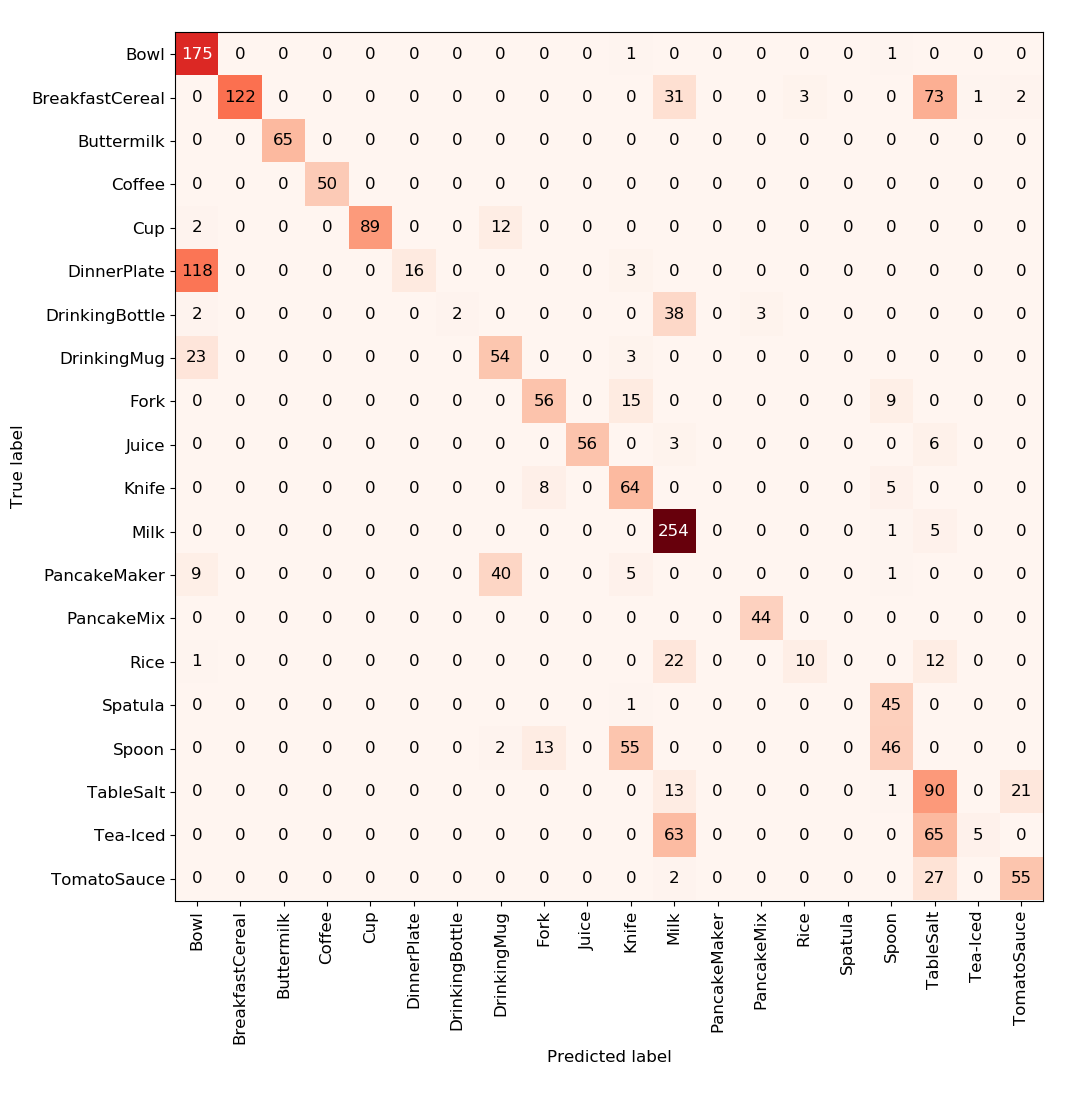
\includegraphics[scale=.315]{img/chapter6/SVMClassifierGTClass.png}
\caption[Konfusionsmatrix der Klassifizierung der Objektklassen durch den SVMAnnotator]{Die Konfusionsmatrix für die Objektklassen Klassifikation der Unreal-Bilder durch den mit echten Bildern trainierten \texttt{SVMAnnotator}.}
\label{fig:SVMClassifierGTClass_confMatrix}
\end{figure}


Die Ergebnisse des \texttt{SVMAnnotators} sind in Abbildung  \ref{fig:SVMClassifierGTClass_confMatrix} zu sehen. Insgesamt sind die Ergebnisse gegenüber dem \texttt{RFAnnotator} etwas besser, da der \texttt{SVMAnnotator} mit 62\% eine etwas höhere \gls{accuracy} aufweist. Jedoch werden vom \texttt{SVMAnnotator} neben dem \textit{Spatula} auch der \textit{PancakeMaker} gar nicht richtig eingeordnet und auch die \textit{DrinkingBottle} schneidet sehr schlecht ab. Der \texttt{SVMAnnotator} ist insgesamt bei einigen Klassen etwas zuverlässiger, hat jedoch auch einige größere Fehlerquellen, was insgesamt zu dem gleichen \gls{f1score} des \texttt{RFAnnotators} von 57\% führt.  

\begin{table}
\centering
\small
\rowcolors{1}{}{lightgray}
\begin{tabularx}{\textwidth}{Xllll}
\textbf{Objekt}	& \textbf{\gls{accuracy}} & \textbf{\gls{precision}}	& \textbf{\gls{recall}}	& \textbf{\gls{f1score}} \\ \hline
Bowl & 0.89 & 0.53 & 0.99 & 0.69 \\  
BreakfastCereal & 0.92 & 1.0 & 0.53 & 0.69 \\  
Buttermilk & 1.0 & 1.0 & 1.0 & 1.0 \\  
Coffee & 1.0 & 1.0 & 1.0 & 1.0 \\  
Cup & 0.99 & 1.0 & 0.86 & 0.93 \\  
DinnerPlate & 0.91 & 1.0 & 0.12 & 0.21 \\  
DrinkingBottle & 0.97 & 1.0 & 0.04 & 0.09 \\  
DrinkingMug & 0.94 & 0.5 & 0.68 & 0.57 \\  
Fork & 0.97 & 0.73 & 0.7 & 0.71 \\  
Juice & 0.99 & 1.0 & 0.86 & 0.93 \\  
Knife & 0.93 & 0.44 & 0.83 & 0.57 \\  
Milk & 0.88 & 0.6 & 0.98 & 0.74 \\  
PancakeMaker & 0.96 & 0.0 & 0.0 & 0.0 \\  
PancakeMix & 1.0 & 0.94 & 1.0 & 0.97 \\  
Rice & 0.97 & 0.77 & 0.22 & 0.34 \\  
Spatula & 0.96 & 0.0 & 0.0 & 0.0 \\  
Spoon & 0.9 & 0.42 & 0.4 & 0.41 \\  
TableSalt & 0.85 & 0.32 & 0.72 & 0.45 \\  
Tea-Iced & 0.91 & 0.83 & 0.04 & 0.07 \\  
TomatoSauce & 0.96 & 0.71 & 0.65 & 0.68 \\    \hline
\textbf{Gesamt}		&	\textbf{0.62}   &	\textbf{0.7}  & \textbf{0.62}     &  \textbf{0.57}     \\
\end{tabularx}
\caption[Objektklassen-spezifische Kenngrößen des SVMAnnotators]{Kenngrößen für die einzelnen Objekte aus der Objektklassen Klassifizierung der Unreal-Bilder mit dem \texttt{SVMAnnotator}.}
\label{tab:SVMClassifierGTClass_metrics}
\end{table}

\subsection{Instanznamen}

\begin{figure}
\centering
	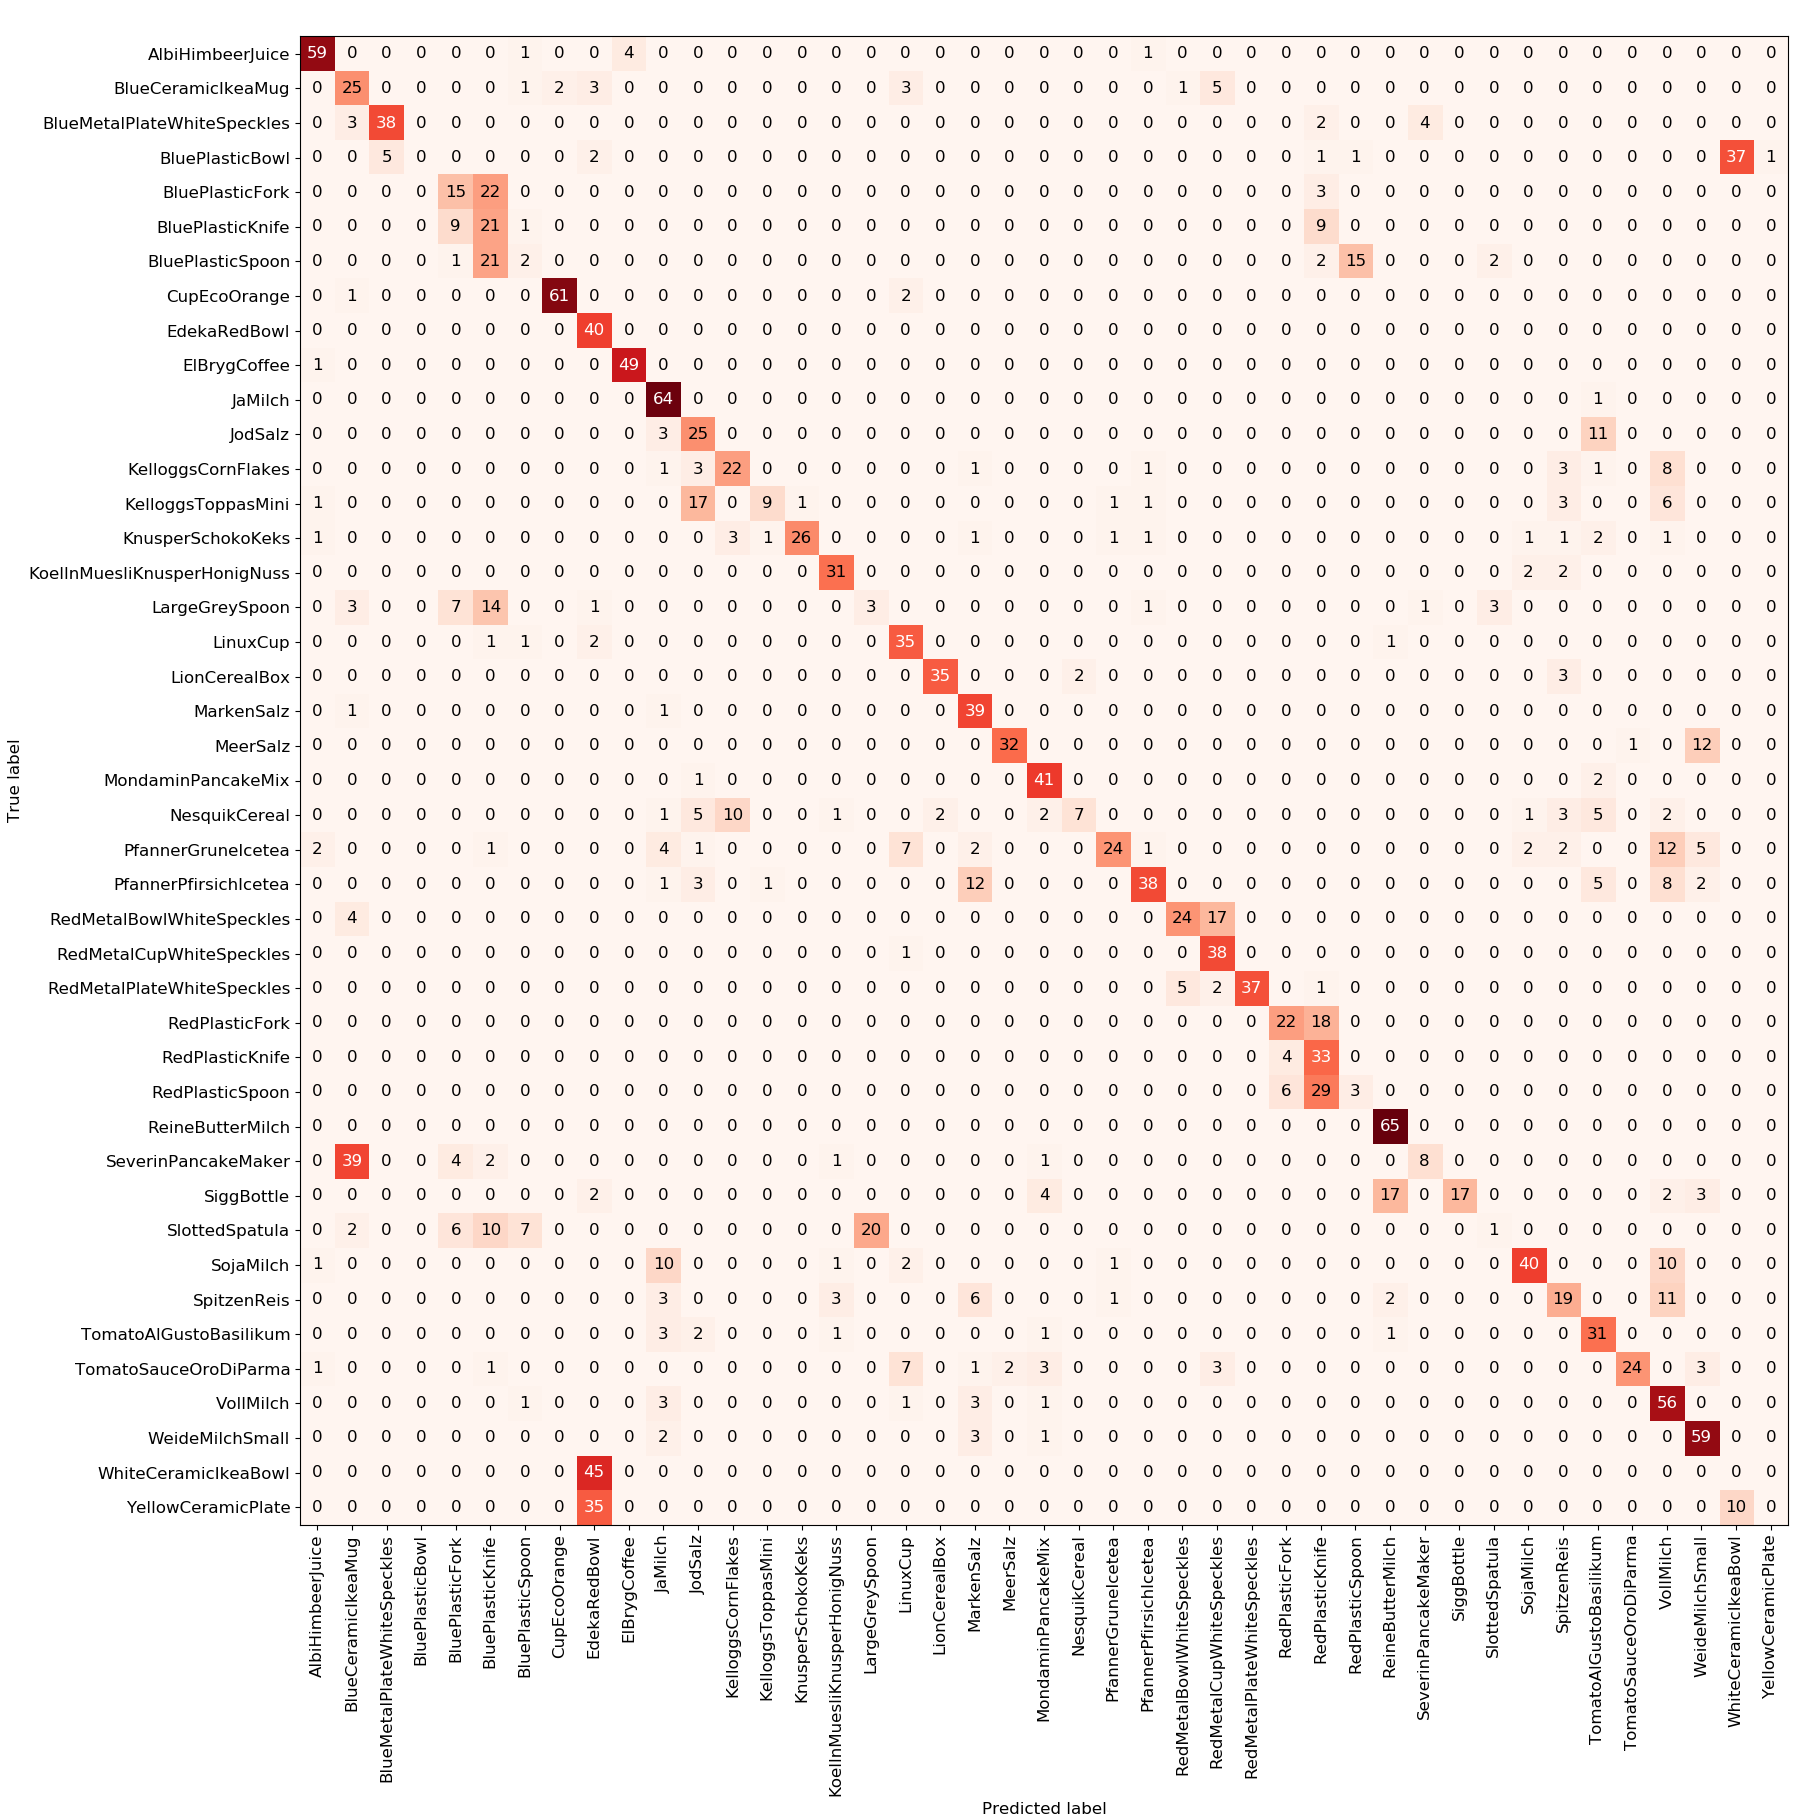
\includegraphics[scale=.292]{img/chapter6/RFClassifierGTInstance.png}
\caption[Konfusionsmatrix der Klassifizierung der Objektinstanzen durch den RFAnnotator]{Die Konfusionsmatrix für die Objektinstanzen Klassifikation der Unreal-Bilder durch den mit echten Bildern trainierten \texttt{RFAnnotator}.}
\label{fig:RFClassifierGTInstance_confMatrix}
\end{figure}

Die Ergebnisse der Instanzenklassifikation des \texttt{RFAnnotators} sind in Abbildung \ref{fig:RFClassifierGTInstance_confMatrix} und Tabelle \ref{tab:RFClassifierGTInstance_metrics} zu finden. Grundsätzlich lässt sich sagen, dass die Klassifikationsrate nahezu identisch ist. Die Fehler bei den Klassen wurden auf die Instanzen übertragen, wodurch nun zu erkennen ist, welche Instanzen die Fehler verursachen. Beispielsweise wird der \textit{SlottedSpatula} in der Hälfte der Fälle für den \textit{LargeGreySpoon} gehalten. Da beide sich ähnlich sehen, ist dies keine Überraschung, zeigt jedoch auch, dass \texttt{RFAnnotator} mit dieser Ähnlichkeit nicht umgehen kann. In den anderen Fällen ist er einem der blauen Geschirrteile zugeordnet, nicht den Roten. \newline
Interessanterweise werden sowohl die \textit{BluePlasticBowl} als auch die \textit{WhiteCeramicIkeaBowl} nicht einmal richtig erkannt. Erstere wird häufig für Letztere gehalten. Die IkeaBowl stattdessen für die \textit{EdekaRedBowl}. Dies fiel bei der Klassifikation mit Objektklassen noch nicht auf, da alle unter \textit{Bowl} zusammengefasst sind und so trotzdem richtig eingeordnet wurden.   

\begin{table}
\centering
\small
\rowcolors{1}{}{lightgray}
\begin{tabularx}{\textwidth}{Xllll}
\textbf{Objekt}	& \textbf{\gls{accuracy}} & \textbf{\gls{precision}}	& \textbf{\gls{recall}}	& \textbf{\gls{f1score}} \\ \hline
AlbiHimbeerJuice & 0.99 & 0.89 & 0.91 & 0.9 \\  
BlueCeramicIkeaMug & 0.95 & 0.32 & 0.63 & 0.42 \\  
BlueMetalPlateWhiteSpeckles & 0.99 & 0.88 & 0.81 & 0.84 \\  
BluePlasticBowl & 0.96 & 0.0 & 0.0 & 0.0 \\  
BluePlasticFork & 0.96 & 0.36 & 0.38 & 0.37 \\  
BluePlasticKnife & 0.93 & 0.23 & 0.53 & 0.32 \\  
BluePlasticSpoon & 0.96 & 0.14 & 0.05 & 0.07 \\  
CupEcoOrange & 1.0 & 0.97 & 0.95 & 0.96 \\  
EdekaRedBowl & 0.93 & 0.31 & 1.0 & 0.47 \\  
ElBrygCoffee & 1.0 & 0.92 & 0.98 & 0.95 \\  
JaMilch & 0.97 & 0.67 & 0.98 & 0.8 \\  
JodSalz & 0.96 & 0.44 & 0.64 & 0.52 \\  
KelloggsCornFlakes & 0.98 & 0.63 & 0.55 & 0.59 \\  
KelloggsToppasMini & 0.97 & 0.82 & 0.23 & 0.36 \\  
KnusperSchokoKeks & 0.99 & 0.96 & 0.67 & 0.79 \\  
KoellnMuesliKnusperHonigNuss & 0.99 & 0.82 & 0.89 & 0.85 \\  
LargeGreySpoon & 0.96 & 0.13 & 0.09 & 0.11 \\  
LinuxCup & 0.98 & 0.6 & 0.88 & 0.71 \\  
LionCerealBox & 0.99 & 0.95 & 0.88 & 0.91 \\  
MarkenSalz & 0.98 & 0.57 & 0.95 & 0.72 \\  
MeerSalz & 0.99 & 0.94 & 0.71 & 0.81 \\  
MondaminPancakeMix & 0.99 & 0.76 & 0.93 & 0.84 \\  
NesquikCereal & 0.97 & 0.78 & 0.18 & 0.29 \\  
PfannerGruneIcetea & 0.97 & 0.86 & 0.38 & 0.53 \\  
PfannerPfirsichIcetea & 0.97 & 0.86 & 0.54 & 0.67 \\  
RedMetalBowlWhiteSpeckles & 0.98 & 0.8 & 0.53 & 0.64 \\  
RedMetalCupWhiteSpeckles & 0.98 & 0.58 & 0.97 & 0.73 \\  
RedMetalPlateWhiteSpeckles & 0.99 & 1.0 & 0.82 & 0.9 \\  
RedPlasticFork & 0.98 & 0.69 & 0.55 & 0.61 \\  
RedPlasticKnife & 0.95 & 0.34 & 0.89 & 0.49 \\  
RedPlasticSpoon & 0.96 & 0.16 & 0.08 & 0.11 \\  
ReineButterMilch & 0.98 & 0.76 & 1.0 & 0.86 \\  
SeverinPancakeMaker & 0.96 & 0.62 & 0.15 & 0.24 \\  
SiggBottle & 0.98 & 1.0 & 0.38 & 0.55 \\  
SlottedSpatula & 0.96 & 0.17 & 0.02 & 0.04 \\  
SojaMilch & 0.98 & 0.87 & 0.62 & 0.72 \\  
SpitzenReis & 0.97 & 0.53 & 0.42 & 0.47 \\  
TomatoAlGustoBasilikum & 0.97 & 0.53 & 0.79 & 0.64 \\  
TomatoSauceOroDiParma & 0.98 & 0.96 & 0.53 & 0.69 \\  
VollMilch & 0.95 & 0.48 & 0.86 & 0.62 \\  
WeideMilchSmall & 0.98 & 0.7 & 0.91 & 0.79 \\  
WhiteCeramicIkeaBowl & 0.93 & 0.0 & 0.0 & 0.0 \\  
YellowCeramicPlate & 0.96 & 0.0 & 0.0 & 0.0 \\   \hline
\textbf{Gesamt}		&	\textbf{0.6}   &	\textbf{0.62}  & \textbf{0.6}     &  \textbf{0.58}     \\
\end{tabularx}
\caption[Objektinstanzen-spezifische Kenngrößen des RFAnnotators]{Kenngrößen für die einzelnen Objekte aus der Objektinstanzen Klassifizierung der Unreal-Bilder mit dem \texttt{RFAnnotator}.}
\label{tab:RFClassifierGTInstance_metrics}
\end{table}

Der \texttt{SVMAnnotator} schneidet bei den Instanzen etwas besser ab als bei den Klassen, dementsprechend auch besser als der \texttt{RFAnnotator} bei den Instanzen. Auch hier sind die Fehler aus der Klassenklassifikation übertragbar. Die \textit{SiggBottle} wird selten erkannt oder als \textit{ReineButterMilch} oder \textit{MondaminPancakeMix} eingeordnet. Zu Verwirrung kommt es hier wahrscheinlich durch deren runde Form und ähnlich helle Farbe. Auch erwähnt seien die sehr schlechten Werte für die beiden farbigen Löffel bei beiden Annotatoren, während die jeweiligen Messer und Gabeln besser abschneiden. Insgesamt sind die Fehlerquellen jedoch wieder nahezu deckungsgleich mit dem \texttt{RFAnnotator}.

\begin{figure}
\centering
	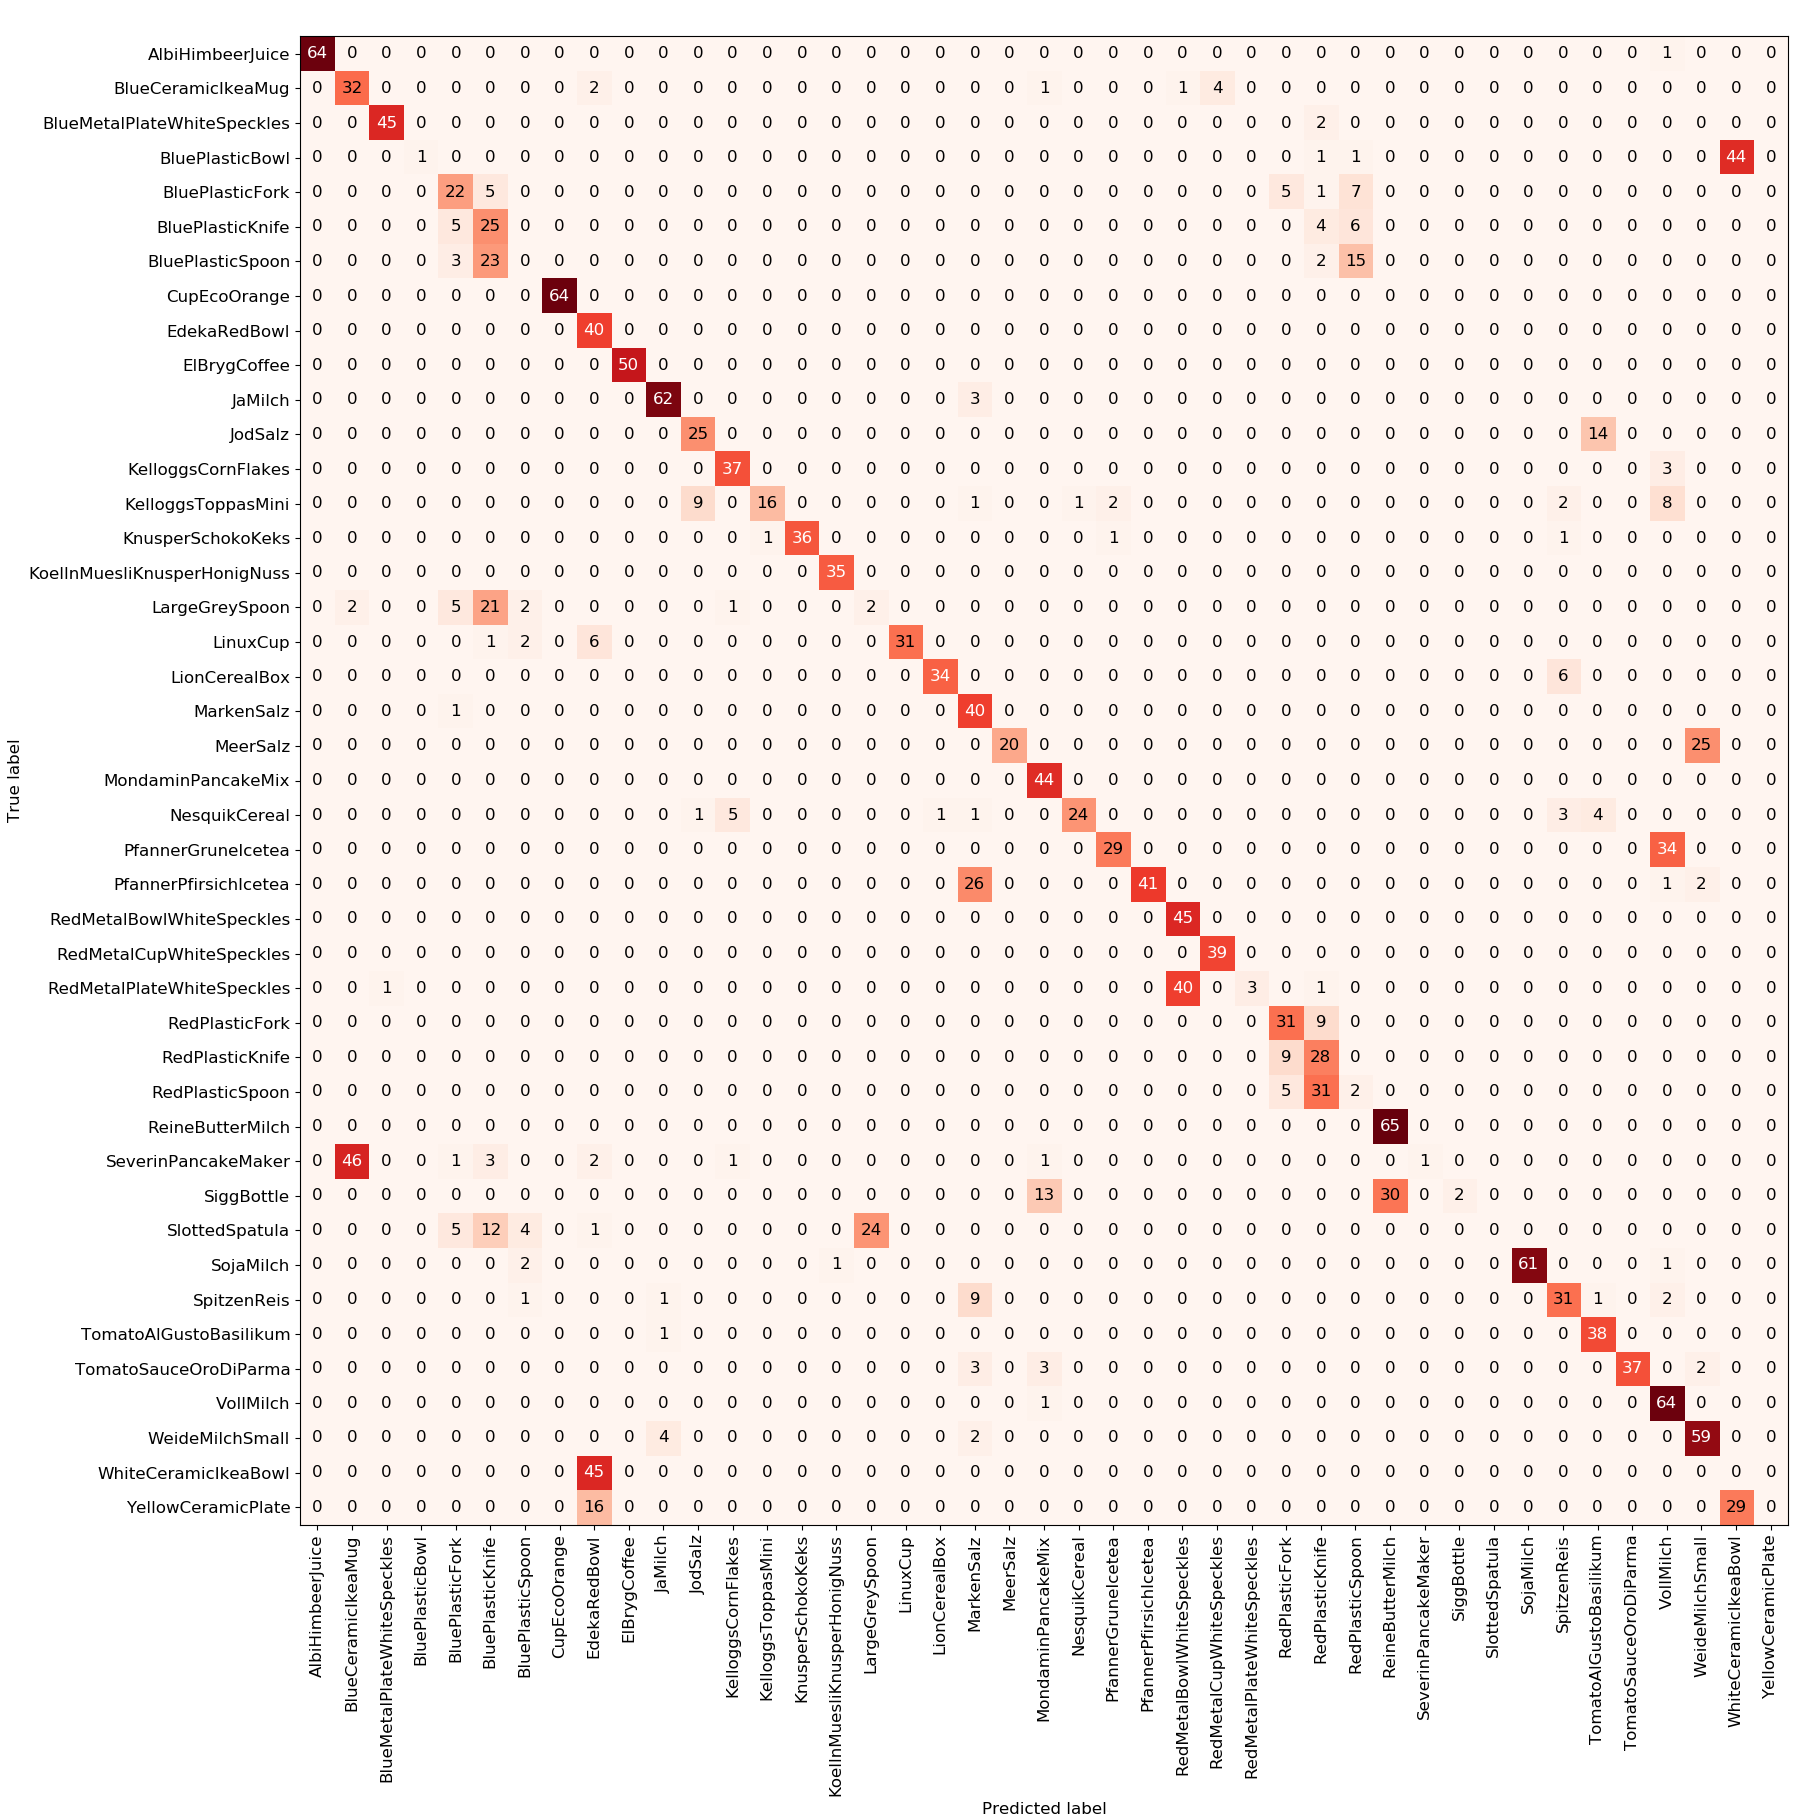
\includegraphics[scale=.292]{img/chapter6/SVMClassifierGTInstance.png}
\caption[Konfusionsmatrix der Klassifizierung der Objektinstanzen durch den SVMAnnotator]{Die Konfusionsmatrix für die Objektinstanzen Klassifikation der Unreal-Bilder durch den mit echten Bildern trainierten \texttt{SVMAnnotator}.}
\label{fig:SVMClassifierGTInstance_confMatrix}
\end{figure}

\begin{table}
\centering
\small
\rowcolors{1}{}{lightgray}
\begin{tabularx}{\textwidth}{Xllll}
\textbf{Objekt}	& \textbf{\gls{accuracy}} & \textbf{\gls{precision}}	& \textbf{\gls{recall}}	& \textbf{\gls{f1score}} \\ \hline
AlbiHimbeerJuice & 1.0 & 1.0 & 0.98 & 0.99 \\  
BlueCeramicIkeaMug & 0.96 & 0.4 & 0.8 & 0.53 \\  
BlueMetalPlateWhiteSpeckles & 1.0 & 0.98 & 0.96 & 0.97 \\  
BluePlasticBowl & 0.97 & 1.0 & 0.02 & 0.04 \\  
BluePlasticFork & 0.97 & 0.52 & 0.55 & 0.54 \\  
BluePlasticKnife & 0.94 & 0.28 & 0.63 & 0.38 \\  
BluePlasticSpoon & 0.96 & 0.0 & 0.0 & 0.0 \\  
CupEcoOrange & 1.0 & 1.0 & 1.0 & 1.0 \\  
EdekaRedBowl & 0.95 & 0.36 & 1.0 & 0.53 \\  
ElBrygCoffee & 1.0 & 1.0 & 1.0 & 1.0 \\  
JaMilch & 0.99 & 0.91 & 0.95 & 0.93 \\  
JodSalz & 0.98 & 0.71 & 0.64 & 0.68 \\  
KelloggsCornFlakes & 0.99 & 0.84 & 0.93 & 0.88 \\  
KelloggsToppasMini & 0.98 & 0.94 & 0.41 & 0.57 \\  
KnusperSchokoKeks & 1.0 & 1.0 & 0.92 & 0.96 \\  
KoellnMuesliKnusperHonigNuss & 1.0 & 0.97 & 1.0 & 0.99 \\  
LargeGreySpoon & 0.96 & 0.08 & 0.06 & 0.07 \\  
LinuxCup & 0.99 & 1.0 & 0.78 & 0.87 \\  
LionCerealBox & 0.99 & 0.97 & 0.85 & 0.91 \\  
MarkenSalz & 0.97 & 0.47 & 0.98 & 0.63 \\  
MeerSalz & 0.98 & 1.0 & 0.44 & 0.62 \\  
MondaminPancakeMix & 0.99 & 0.7 & 1.0 & 0.82 \\  
NesquikCereal & 0.99 & 0.96 & 0.62 & 0.75 \\  
PfannerGruneIcetea & 0.97 & 0.91 & 0.46 & 0.61 \\  
PfannerPfirsichIcetea & 0.98 & 1.0 & 0.59 & 0.74 \\  
RedMetalBowlWhiteSpeckles & 0.97 & 0.52 & 1.0 & 0.69 \\  
RedMetalCupWhiteSpeckles & 1.0 & 0.91 & 1.0 & 0.95 \\  
RedMetalPlateWhiteSpeckles & 0.97 & 1.0 & 0.07 & 0.13 \\  
RedPlasticFork & 0.98 & 0.62 & 0.78 & 0.69 \\  
RedPlasticKnife & 0.96 & 0.35 & 0.76 & 0.48 \\  
RedPlasticSpoon & 0.95 & 0.06 & 0.05 & 0.06 \\  
ReineButterMilch & 0.98 & 0.68 & 1.0 & 0.81 \\  
SeverinPancakeMaker & 0.96 & 1.0 & 0.02 & 0.04 \\  
SiggBottle & 0.97 & 1.0 & 0.04 & 0.09 \\  
SlottedSpatula & 0.97 & 0.0 & 0.0 & 0.0 \\  
SojaMilch & 1.0 & 1.0 & 0.94 & 0.97 \\  
SpitzenReis & 0.98 & 0.72 & 0.69 & 0.7 \\  
TomatoAlGustoBasilikum & 0.99 & 0.67 & 0.97 & 0.79 \\  
TomatoSauceOroDiParma & 0.99 & 1.0 & 0.82 & 0.9 \\  
VollMilch & 0.96 & 0.56 & 0.98 & 0.72 \\  
WeideMilchSmall & 0.97 & 0.67 & 0.91 & 0.77 \\  
WhiteCeramicIkeaBowl & 0.92 & 0.0 & 0.0 & 0.0 \\  
YellowCeramicPlate & 0.97 & 0.0 & 0.0 & 0.0 \\      \hline
\textbf{Gesamt}		&	\textbf{0.66}   &	\textbf{0.72}  & \textbf{0.66}     &  \textbf{0.62}     \\
\end{tabularx}
\caption[Objektinstanzen-spezifische Kenngrößen des SVMAnnotators]{Kenngrößen für die einzelnen Objekte aus der Objektinstanzen Klassifizierung der Unreal-Bilder mit dem \texttt{SVMAnnotator}.}
\label{tab:SVMClassifierGTInstance_metrics}
\end{table}


\section{10-fache Kreuzvalidierung der Unreal-Bilder mit MLNs}
\label{sec:onlyUnrealImages}
Im Folgenden werden nur Unreal-Bilder zum Trainieren und Testen eines \gls{mln} verwendet. Als \gls{gt} dienen die Objektklassen oder Instanznamen. Die logischen Prädikate wurden dazu mit der in Kapitel \ref{sec:analysisengine} vorgestellten \gls{ae} aus den 570 Unreal-Bildern extrahiert. Diese werden, wie in Tabelle \ref{tab:annotators} auf S.\pageref{tab:annotators} beschrieben, für das Modell deklariert.  Zusätzlich gibt es noch das $scene$-Prädikat und eine Einschränkung für das $object$-Prädikat:
\begin{itemize}
\item das $scene(scene)$ Prädikat ordnet die Szene in einen räumlichen Kontext ein. Die Domäne für das Prädikat ist $dom(scene) = \{breakfast, cooking, fridge\}$
\item das Prädikat $object$ wird folgendermaßen definiert: $object(cluster, object!)$, und beschreibt die \gls{gt} des Clusters. Der \glqq!\grqq \ Operator besagt, dass dieses Prädikat als funktionelle Einschränkung behandelt werden soll. Das bedeutet, dass immer exakt ein Atom wahr sein muss; alle anderen sind falsch.\footnote{\url{http://pracmln.org/mln_syntax.html}} Im Falle des obigen Prädikats bedeutet das, dass jedem Cluster genau eine \gls{gt} zugeordnet sein muss. Dies macht im Rahmen des Modells Sinn, da ein Objekt nicht mehreren Klassen zugleich angehören kann und wurde auch in \cite{pr2looking} in der \gls{mln}-Deklaration angenommen.
\end{itemize}
Das folgende \gls{mln} beschreibt die Zusammenhänge der einzelnen Informationen der Annotatoren und der Objektklassen:
\begin{align*}
& w_{1} \ shape(?c, +?sha) \wedge object(?c, +?obj) \\
& w_{2} \ color(?c, +?col) \wedge object(?c, +?obj) \\
& w_{3} \ size(?c, +?size) \wedge object(?c, +?obj) \\
& w_{4} \ instance(?c, +?inst) \wedge object(?c, +?obj) \\
& w_{5} \ goggles\_Logo(?c, +?comp) \wedge object(?c, +?obj)\\
& w_{6} \ goggles\_Text(?c, +?text) \wedge object(?c, +?obj)\\
& w_{7} \ goggles\_Product(?c, +?prod) \wedge object(?c, +?obj)\\
& w_{8} \ scene(+?s) \wedge object(?c, +?obj)\\
& w_{9} \ object(?c1, +?t1) \wedge object(?c2, +?t2) \wedge ?c1 =/= ?c2
\end{align*}
\textit{Hinweise zur Syntax von \pracmln:} Jeder Variable muss ein \glqq ?\grqq \ vorangestellt werden. Das \glqq +\grqq \ bedeutet, dass für jedes Element der Domäne dieser Variable eine Formel erstellt wird. \footnote{\url{http://pracmln.org/mln_syntax.html}}  \par
 
Ein \gls{mln} wurde mit \textit{Discriminative Pseudo-likelihood Learning with Custom Grounding} trainiert. Es wurde die \textit{Discrimitive} Variante des Lernalgorithmus gewählt, da es ein genaueres Modell und geringeren Rechenaufwand bietet. Als Voraussetzung müssen bestimmte Prädikate bei den Anfragen entweder nur in den Anfragen oder der Evidenzen vorkommen. Da die Objekte in diesem Fall nach ihrer \gls{gt} klassifiziert werden sollen, wird nur nach dem $object$-Prädikat gefragt werden. Die \textit{Custom Grounding} Variante bietet eine schnellere Rechenzeit, wenn die Formeln größtenteils aus Konjunktionen bestehen. Eine Regularisierung findet durch den Gaussian-Prior mit einem Mittelwert $\mu = 0$ und einer Standardabweichung $\sigma = 10$ statt. \par   

Zum Testen werden Anfragen, um welche Objekte es sich bei den Clustern handelt, an das trainierte \gls{mln} gestellt. Es soll also die bedingte Wahrscheinlichkeit $P(object \mid E)$ berechnet werden. Es wird eine Evidenz angegeben, die von der Form her den Trainingsdaten entspricht, also eine wahrgenommene Szene darstellt. Nur das $object$-Prädikat wurde entfernt, da die Objektklasse sonst schon bekannt wäre und nicht aus den anderen Eigenschaften darauf geschlossen werden muss. Als Inferenzmechanismus wird \textit{WCSP} verwendet. Dies ist ein Algorithmus, der die \textit{Most Probable Explanation (MPE)} berechnet, also nicht die gesamte bedingte Wahrscheinlichkeit, sondern nur die wahrscheinlichste Variablenbelegung unter Bedingung der Evidenz. WCSP wandelt dazu das instanziierte \gls{mn} in ein \textit{gewichtetes Constraint Satisfaction Problem} um. \par

\begin{figure}
\centering
	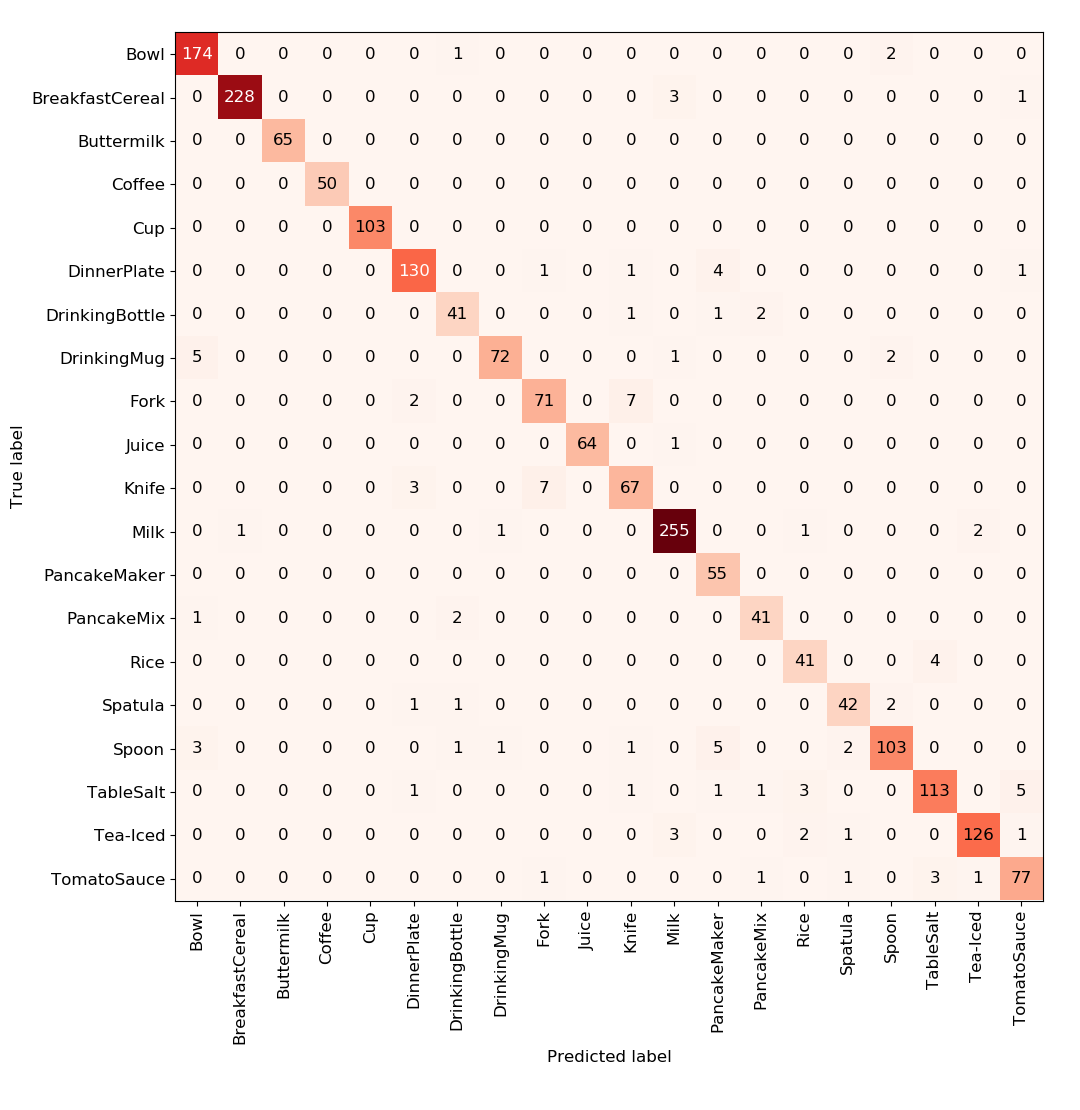
\includegraphics[scale=.315]{img/chapter6/UnrealGTClass.png}
\caption[Konfusionsmatrix des gesamten Unreal-Bilder Datensatzes mit Objektklassen als GT]{Die Konfusionsmatrix für die 10-fache Kreuzvalidierung der gesamten 570 Unreal-Bilder. Als \gls{gt} fungierten die Objektklassen.}
\label{fig:UnrealGTClass_confMatrix}
\end{figure}

Um dieses Modell zu evaluieren, wird 10-fache Kreuzvalidierung durchgeführt. Dabei wird der gesamte Datensatz, also alle 570 Bilder, in 10 Teilmengen aufgeteilt. Jedes Bild bleibt für den gesamten Prozess in seiner Teilmenge. Nun werden 9 Teilmengen als Trainingsdaten für ein \gls{mln} benutzt, während die übrige 10. Teilmenge zum Testen zur Verfügung steht. Dieser Vorgang wird 10 mal durchgeführt, sodass jede Teilmenge genau einmal zum Testen verwendet wurde. Die Ergebnisse der einzelnen Durchgänge können nun gemittelt werden. Dies verhindert die Überanpassung des Modells, also die Anpassung an die Trainingsdaten und damit einen Verlust der Generalität des Modells. \par

\subsection{Objektklassen}

\begin{table}
\centering
\small
\rowcolors{1}{}{lightgray}
\begin{tabularx}{\textwidth}{Xllll}
\textbf{Objekt}	& \textbf{\gls{accuracy}} & \textbf{\gls{precision}}	& \textbf{\gls{recall}}	& \textbf{\gls{f1score}} \\ \hline
Bowl & 0.99 & 0.95 & 0.98 & 0.97 \\  
BreakfastCereal & 1.0 & 1.0 & 0.98 & 0.99 \\  
Buttermilk & 1.0 & 1.0 & 1.0 & 1.0 \\  
Coffee & 1.0 & 1.0 & 1.0 & 1.0 \\  
Cup & 1.0 & 1.0 & 1.0 & 1.0 \\  
DinnerPlate & 0.99 & 0.95 & 0.95 & 0.95 \\  
DrinkingBottle & 1.0 & 0.89 & 0.91 & 0.9 \\  
DrinkingMug & 0.99 & 0.97 & 0.9 & 0.94 \\  
Fork & 0.99 & 0.89 & 0.89 & 0.89 \\  
Juice & 1.0 & 1.0 & 0.98 & 0.99 \\  
Knife & 0.99 & 0.86 & 0.87 & 0.86 \\  
Milk & 0.99 & 0.97 & 0.98 & 0.98 \\  
PancakeMaker & 0.99 & 0.83 & 1.0 & 0.91 \\  
PancakeMix & 1.0 & 0.91 & 0.93 & 0.92 \\  
Rice & 0.99 & 0.87 & 0.91 & 0.89 \\  
Spatula & 1.0 & 0.91 & 0.91 & 0.91 \\  
Spoon & 0.99 & 0.94 & 0.89 & 0.92 \\  
TableSalt & 0.99 & 0.94 & 0.9 & 0.92 \\  
Tea-Iced & 0.99 & 0.98 & 0.95 & 0.96 \\  
TomatoSauce & 0.99 & 0.91 & 0.92 & 0.91 \\  \hline
\textbf{Gesamt}		&	\textbf{0.95}   &	\textbf{0.95}  & \textbf{0.95}     &  \textbf{0.95}    \\
\end{tabularx}
\caption[Objektklassen-spezifische Kenngrößen des gesamten Unreal-Bilder Datensatzes]{Kenngrößen für die einzelnen Objekte aus der 10-fachen Kreuzvalidierung der gesamten Unreal-Bilder. Die Objektklassen sind die \gls{gt}.}
\label{tab:UnrealGTClass_metrics}
\end{table}

Die Ergebnisse der Kreuzvalidierung mit Objektklassen als \gls{gt} sind in Abbildung \ref{fig:UnrealGTClass_confMatrix} und Tabelle \ref{tab:UnrealGTClass_metrics} dargestellt. Insgesamt werden eine hohe \gls{accuracy} für alle Objektklassen als auch Werte über 90\% für \gls{precision}, \gls{recall} und \gls{f1score} erreicht. Einzig das Besteck und der Reis schneiden etwas schlechter ab. Bei dem Besteck war dies erwartet worden, da \textit{Knifes}, \textit{Forks} und \textit{Spoons} kleiner  als viele andere Objekte und damit visuelle Eigenschaften schwieriger auszumachen sind. Im Gegensatz zu den Ergebnissen der \glspl{klassifikator} ist eine deutliche Verbesserung zu erkennen. Vor allem werden keine Objekte gar nicht erkannt. Die bessere Klassifikationsrate war jedoch erwartet worden, da \glspl{mln} die Ergebnisse verschiedener Experten, die Annotatoren in \robosherlock, kombiniert und solche Ensembles, wie bereits zuvor dargelegt, zu besseren Ergebnissen kommen können. \newline
Um zu beweisen, dass dies auch hier der Fall ist, sind in den Abbildungen \ref{fig:singleEvidences} und \ref{fig:singleEvidencesGog} sind die Ergebnisse der 10-fachen Kreuzvalidierung mit nur jeweils einem Prädikat abgebildet. Dazu wurden die \glspl{mln} mit nur einem Prädikat von \robosherlock und dem $scene$-Prädikat trainiert und befragt. \newline
Es ist zu erkennen, dass bei Farbe, Form und Größe einige bestimmte Objekte präferiert werden. Die Anzahl der präferierten Objekte korrespondiert stark mit der Anzahl der möglichen Atome für jedes Prädikat. Es gibt zum Beispiel 10 Atome für Farbe und in der Konfusionsmatrix 9-10 Objekte, die regelmäßig klassifiziert werden. Bei der Form scheinen sich die 3 Atome auf je circa 2 Objekte zu verteilen: \textit{Fork}, \textit{Knife}, \textit{Spoon} für $small$, \textit{Tea-Iced} und \textit{DrinkingBottle} für $medium$ und \textit{PancakeMaker} und \textit{Tea-Iced} für $large$. Bei der Instanz fällt auf, dass vieles als \textit{Spoon} eingeordnet wird, während aber viele andere Objekt richtig zugeordnet sind. Diese Neigung war bei dem für die Instanz verantwortlichen \texttt{SVMAnnotator} in den vorherigen Experimenten interessanterweise nicht zu erkennen. Insgesamt scheinen sich die Fehler des \texttt{SVMAnnotators} im \gls{mln} nicht zu wiederholen, stattdessen tun sich andere auf. Der \texttt{GogglesAnnotator} hat sehr gute Ergebnisse auf texturierten oder beschrifteten Objekten. Insgesamt unterstützen diese Ergebnisse die Idee einer besseren Erkennung durch Ensembles, da jeder Annotator seine Stärken und Schwächen aufweist, und erst durch die Zusammenführung der einzelnen Ergebnisse eine gute Klassifikationsrate erreicht wird.\par

\begin{figure}
\centering
	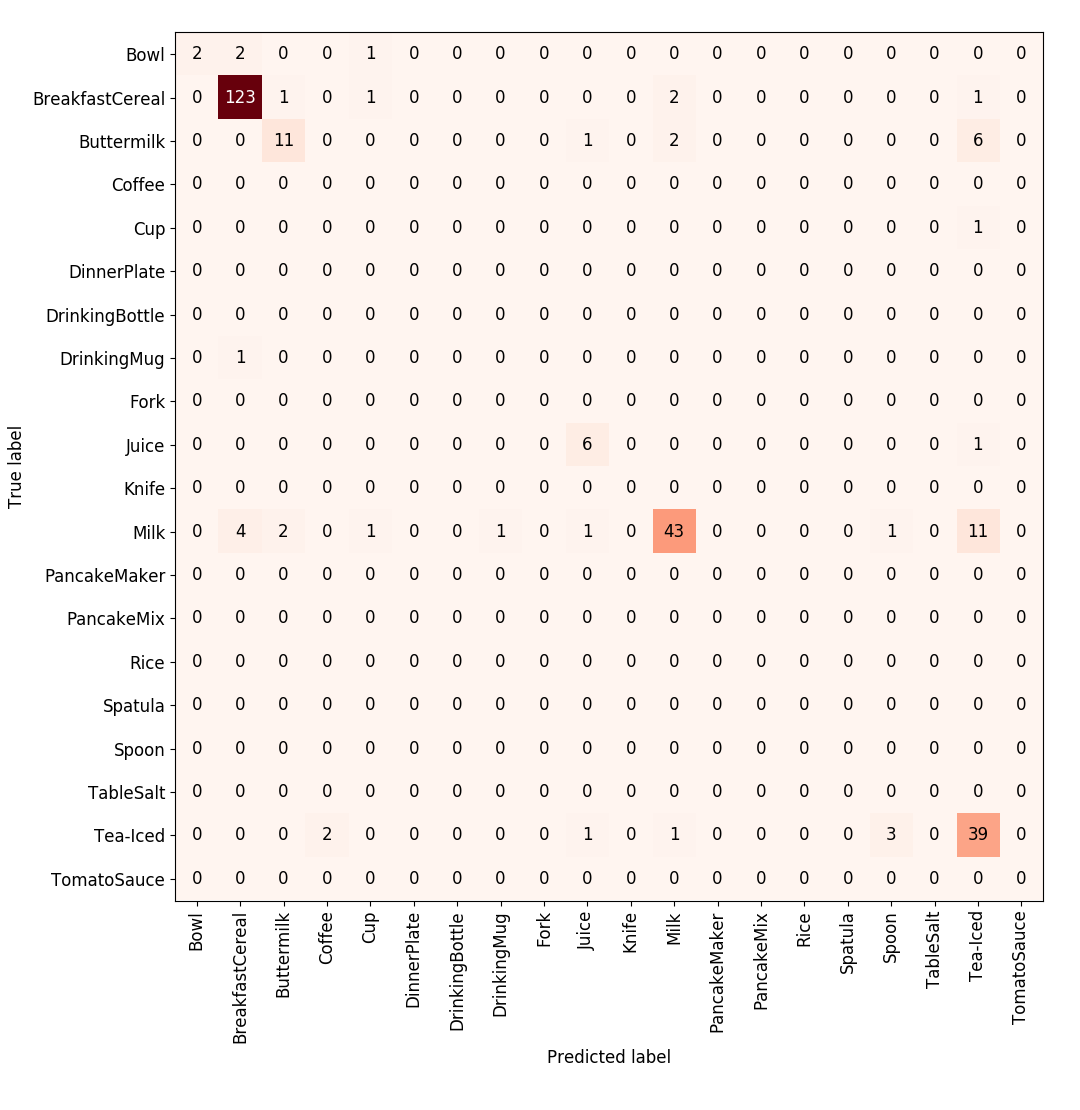
\includegraphics[scale=.27]{img/chapter6/UnrealGTClass_goggles.png}	
\caption[Konfusionsmatrix für die Klassifikation nur durch den \texttt{GogglesAnnotator}]{Konfusionsmatrix für die 10-fache Kreuzvalidierung der Unreal-Bilder, wobei nur die \texttt{GogglesAnnotator} und $scene$-Prädikate zum Trainieren und Testen verwendet wurden.}
\label{fig:singleEvidencesGog}
\end{figure}

\begin{figure}
\centering
	\begin{subfigure}[b]{0.48\textwidth}
		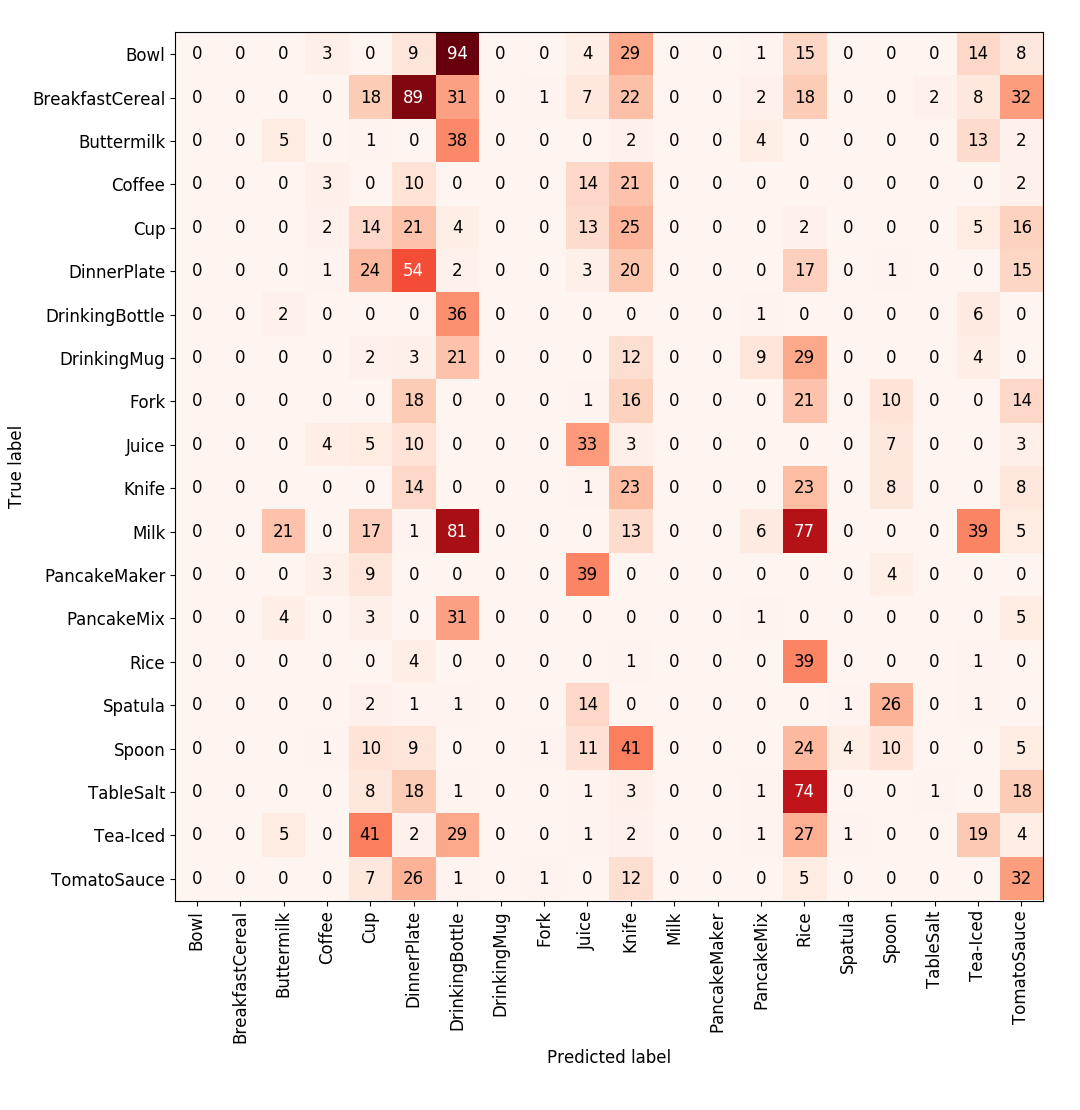
\includegraphics[scale=.27]{img/chapter6/UnrealGTClass_color.png}
		\subcaption{Farbe}
	\end{subfigure}
	\begin{subfigure}[b]{0.48\textwidth}
		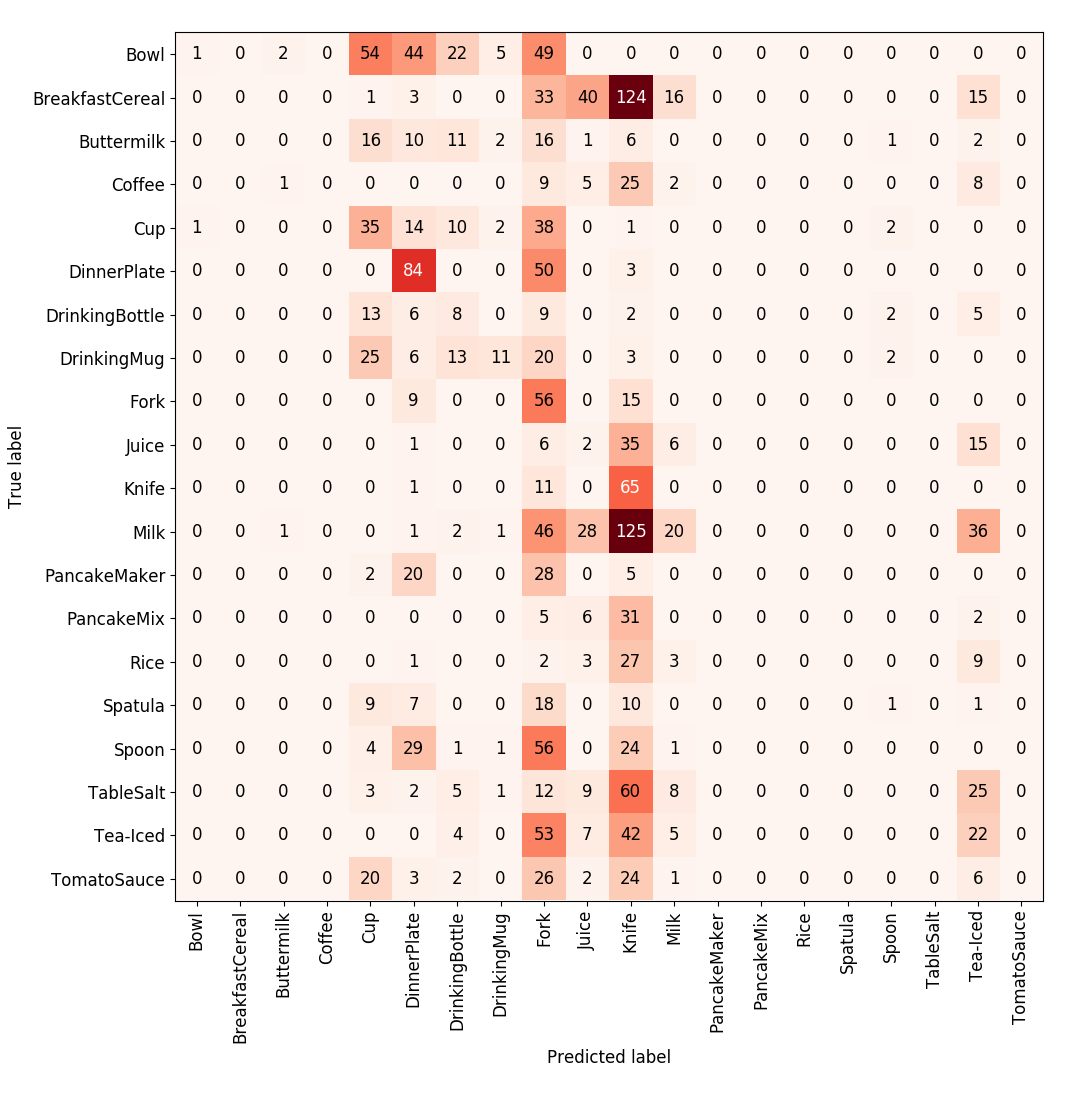
\includegraphics[scale=.27]{img/chapter6/UnrealGTClass_shape.png}	
		\subcaption{Form}
	\end{subfigure}
	\begin{subfigure}[b]{0.48\textwidth}
		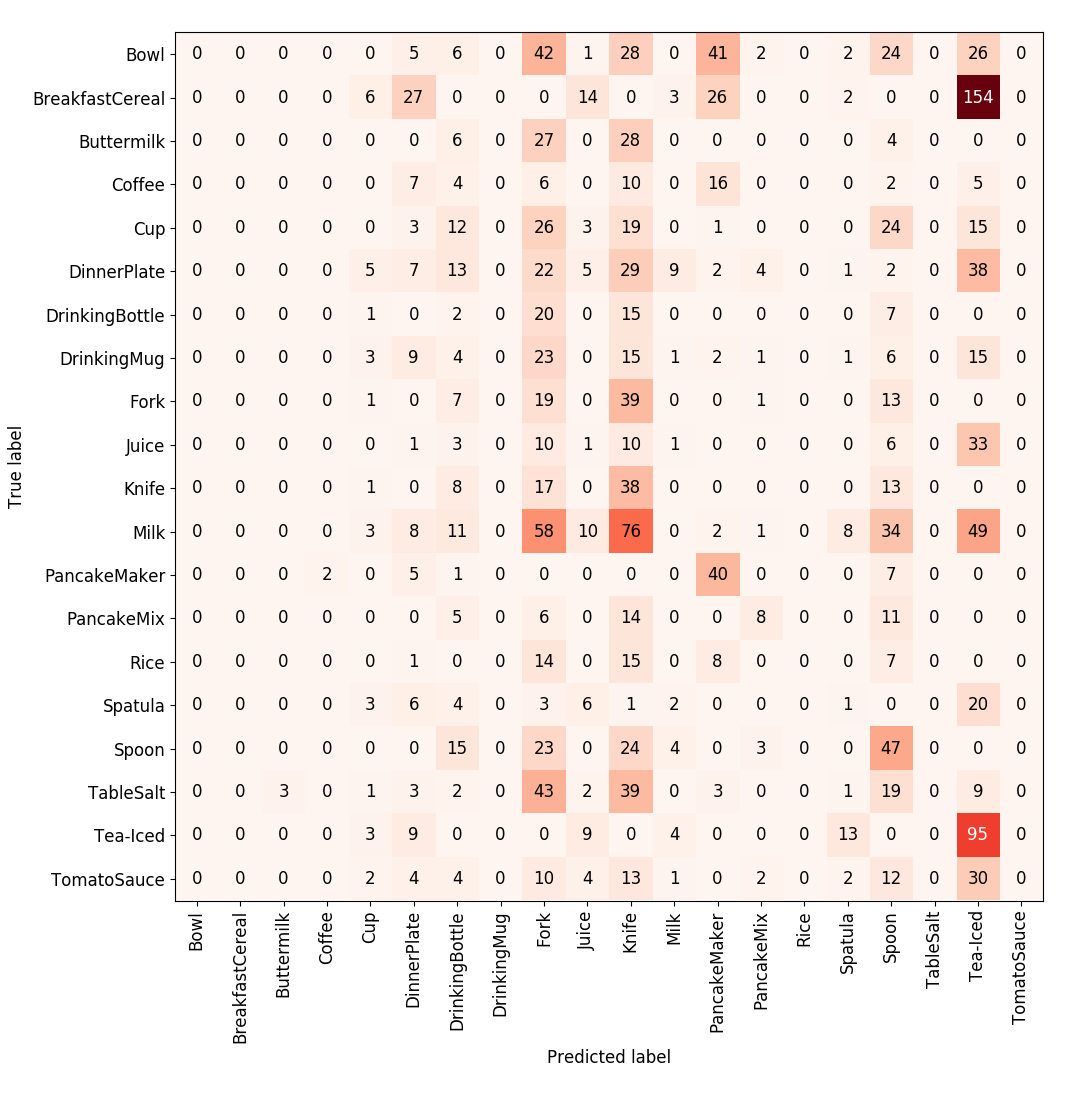
\includegraphics[scale=.27]{img/chapter6/UnrealGTClass_size.png}	
		\subcaption{Größe}
	\end{subfigure}
	\begin{subfigure}[b]{0.48\textwidth}
		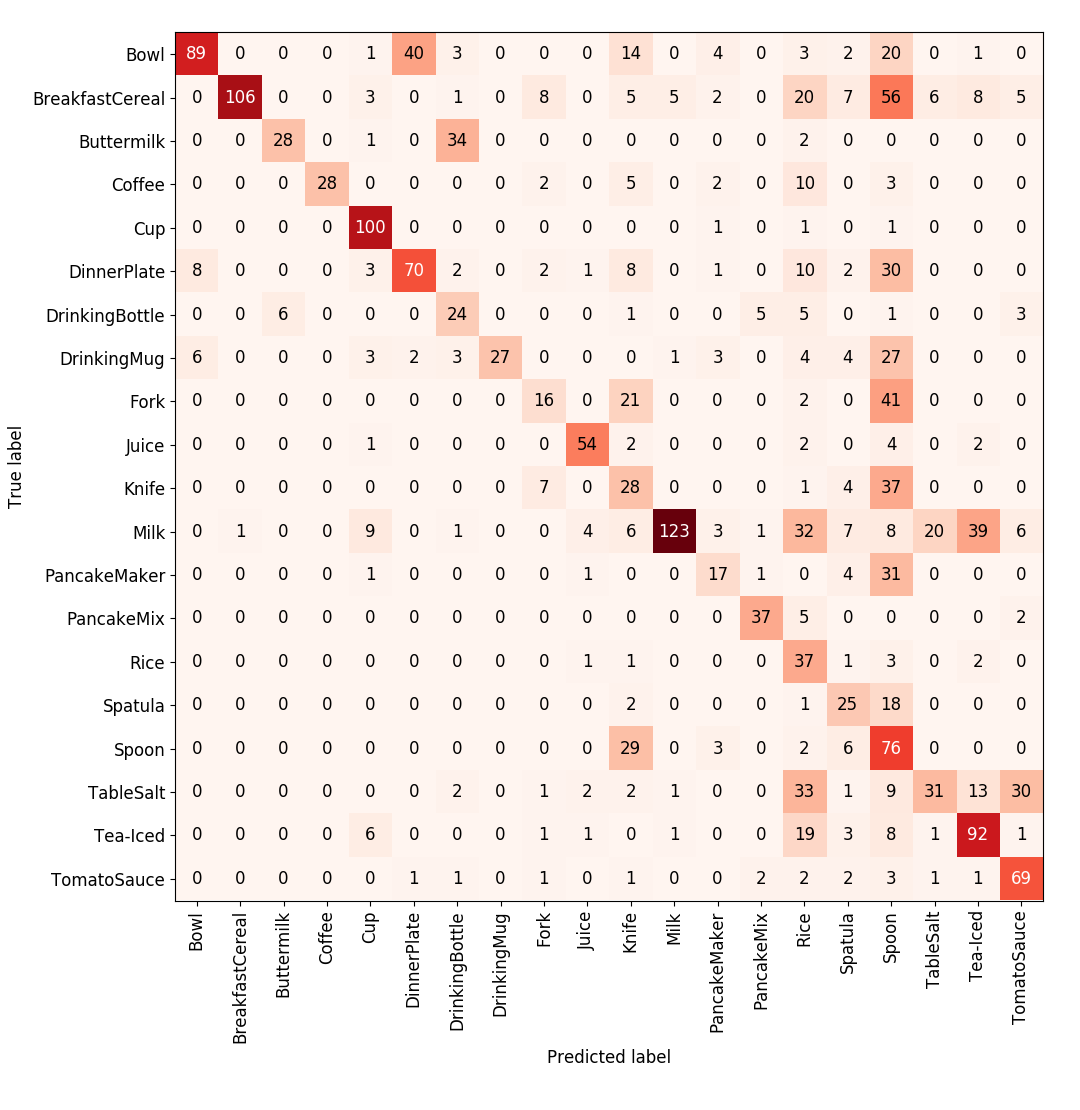
\includegraphics[scale=.27]{img/chapter6/UnrealGTClass_instance.png}	
		\subcaption{Instanz}
	\end{subfigure}
\caption[Konfusionsmatrizen für die Klassifikation mit nur einem Annotatoren Prädikat]{Konfusionsmatrizen der 10-fachen Kreuzvalidierung des gesamten Unreal-Bilder Satzes, wobei nur ein \robosherlock Prädikat (Form, Farbe, Größe, Instanz) und das $scene$-Prädikat zum Trainieren und Testen verwendet wurde.}
\label{fig:singleEvidences}
\end{figure}

\subsection{Instanznamen}

Die Ergebnisse der 10-fachen Kreuzvalidierung mit Instanznamen als \gls{gt} sind in Abbildung \ref{fig:UnrealGTInstance_confMatrix} und Tabelle \ref{tab:UnrealGTInstance_metrics} einzusehen. Wieder werden Werte über 90\% für fast alle Objekte erreicht. Ausnahmen bilden das rote Besteck, der \textit{SeverinPancakeMaker} und der \textit{LargeGreySpoon}. Letzterer wird häufig als besagter PancakeMaker eingestuft, während der PancakeMaker selber meistens durchaus korrekt klassifiziert wird (zu sehen am hohen \gls{recall} gegenüber der \gls{precision}). Dass41elbe konnte für den \textit{SeverinPancakeMaker} und seine Klasse \textit{PancakeMaker} auch schon bei der Klassifikation der Objektklassen beobachtet werden. Bei den \glspl{klassifikator} verhielt es sich dagegen genau anderes herum. Zwei der roten Besteckteile, die \textit{RedPlasticFork} und das \textit{RedPlasticKnife}, liegen mit \gls{precision}, \gls{recall} und \gls{f1score} von unter 80\% deutlich unter dem Mittel der anderen Objekte und auch unter dem des anderen Bestecks. Denn selbst die blauen Gegenstücke, die \textit{BluePlasticFork} und das \textit{BluePlasticKnife}, erreichen Werte über 90\%.

\begin{figure}
\centering
	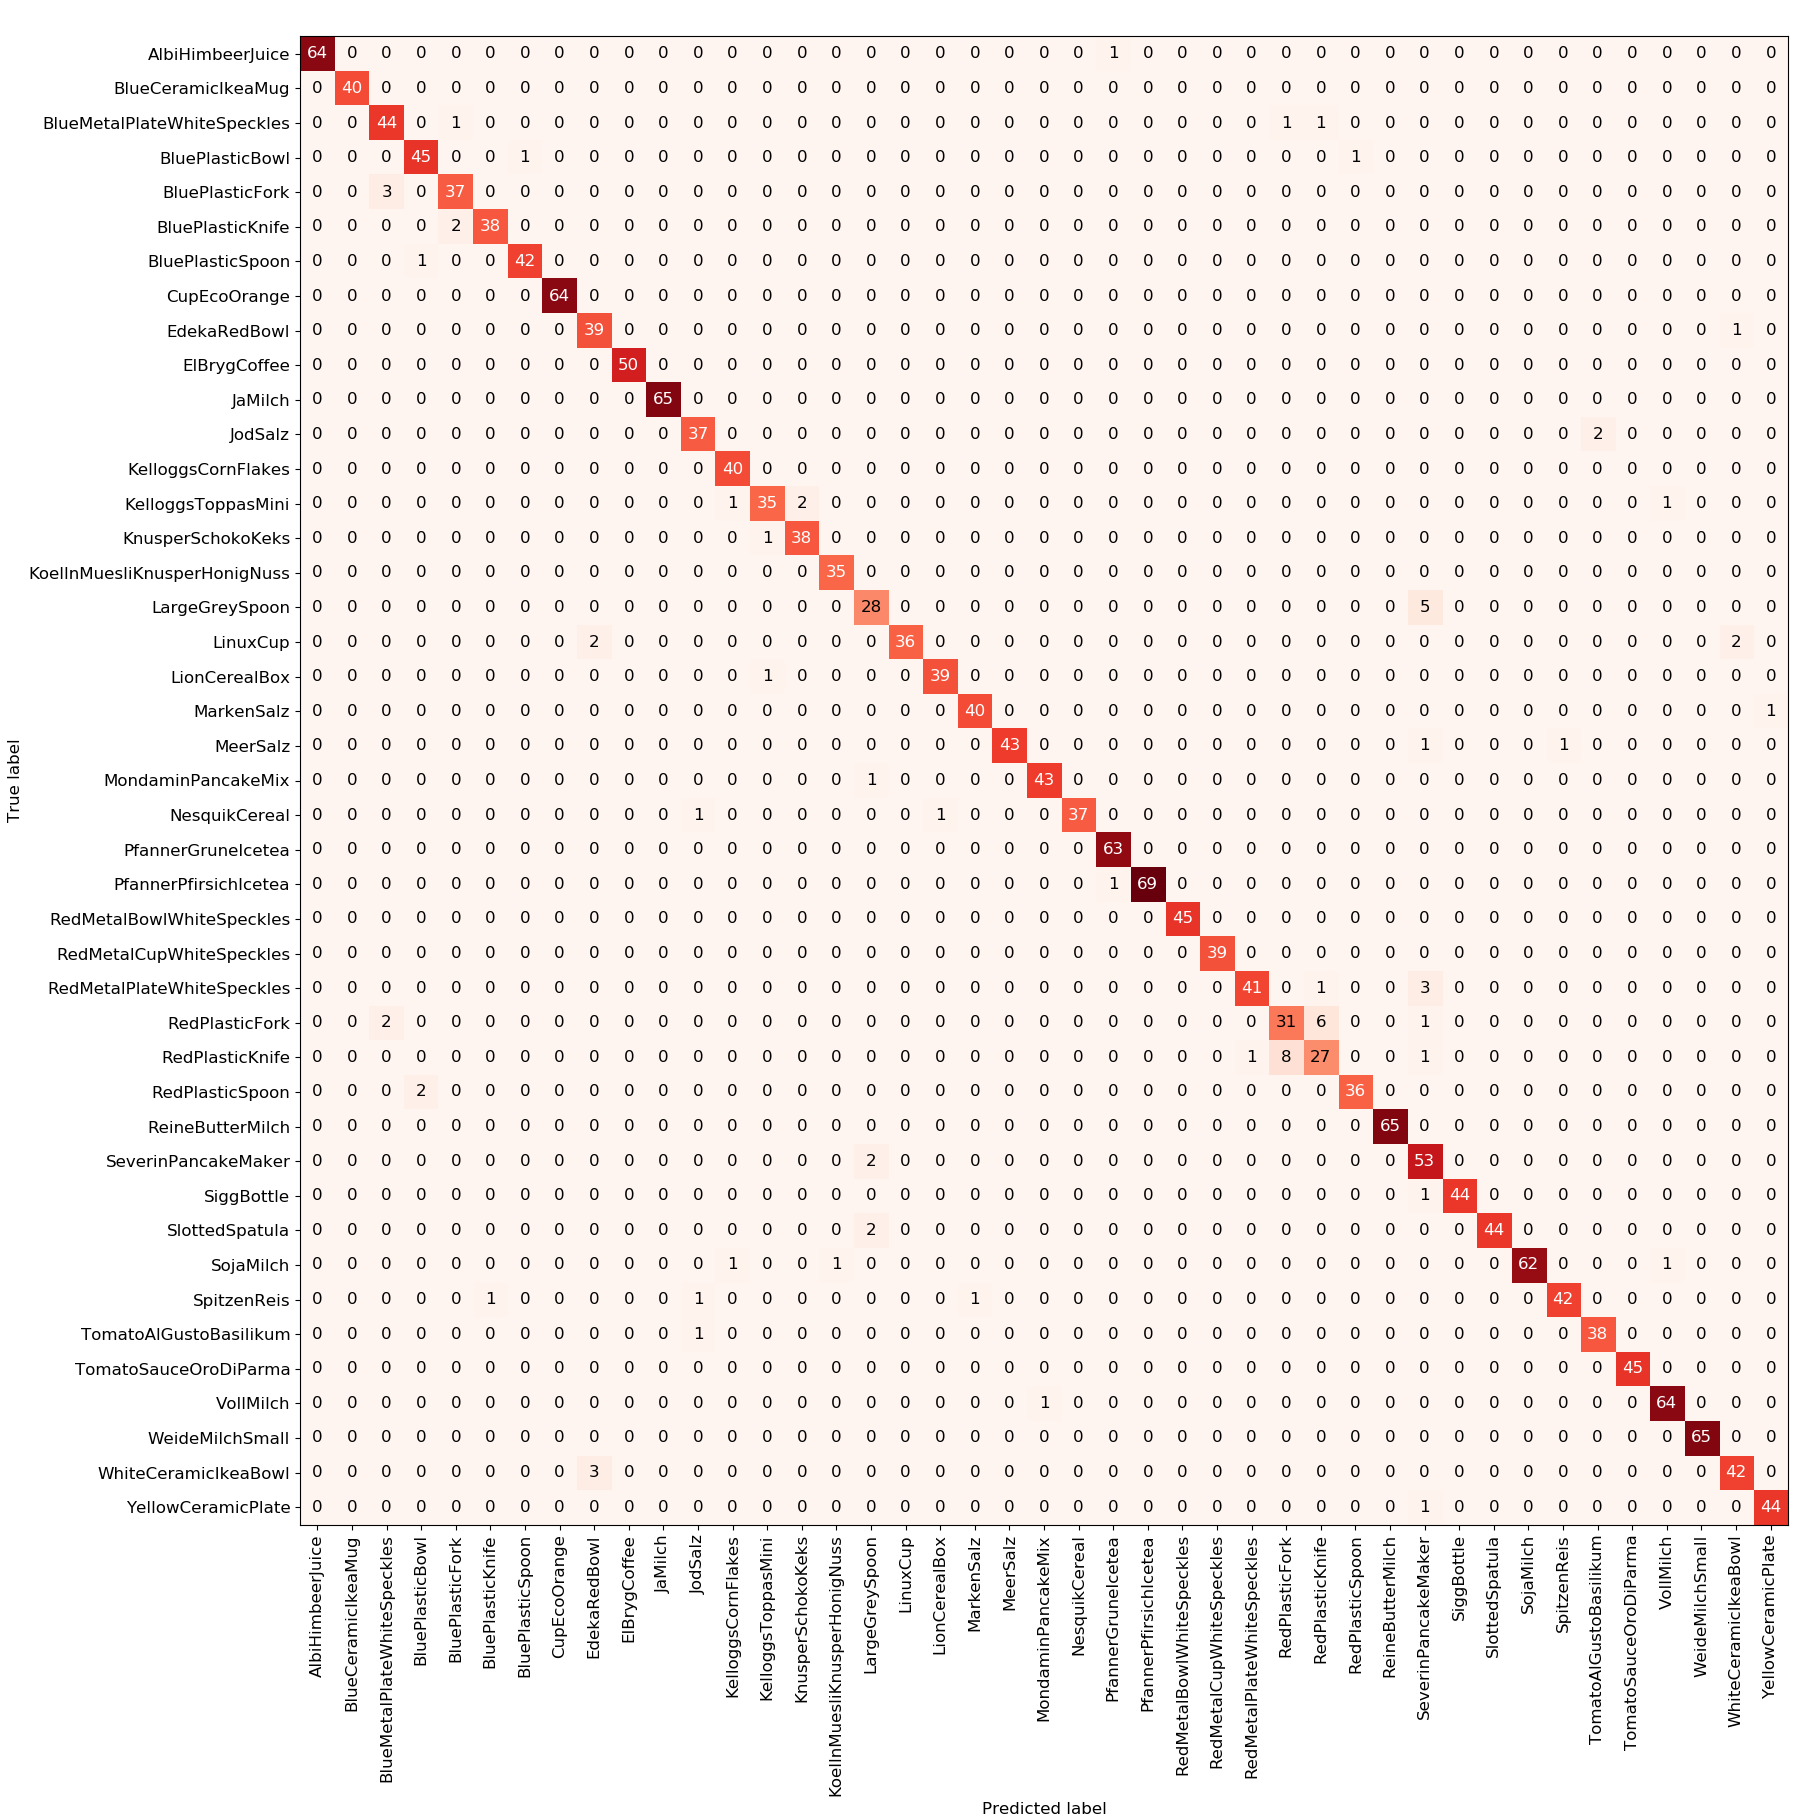
\includegraphics[scale=.292]{img/chapter6/UnrealGTInstance.png}
\caption[Konfusionsmatrix des gesamten Unreal-Bilder Datensatzes mit den Instanznamen als GT]{Die Konfusionsmatrix für die 10-fache Kreuzvalidierung der gesamten 570 Unreal-Bilder. Die \gls{gt} sind die Instanznamen.}
\label{fig:UnrealGTInstance_confMatrix}
\end{figure}

\begin{table}
\centering
\small
\rowcolors{1}{}{lightgray}
\begin{tabularx}{\textwidth}{Xllll}
\textbf{Objekt}	& \textbf{\gls{accuracy}} & \textbf{\gls{precision}}	& \textbf{\gls{recall}}	& \textbf{\gls{f1score}} \\ \hline
AlbiHimbeerJuice & 1.0 & 1.0 & 0.98 & 0.99 \\  
BlueCeramicIkeaMug & 1.0 & 1.0 & 1.0 & 1.0 \\  
BlueMetalPlateWhiteSpeckles & 1.0 & 0.9 & 0.94 & 0.92 \\  
BluePlasticBowl & 1.0 & 0.94 & 0.96 & 0.95 \\  
BluePlasticFork & 1.0 & 0.93 & 0.93 & 0.93 \\  
BluePlasticKnife & 1.0 & 0.97 & 0.95 & 0.96 \\  
BluePlasticSpoon & 1.0 & 0.98 & 0.98 & 0.98 \\  
CupEcoOrange & 1.0 & 1.0 & 1.0 & 1.0 \\  
EdekaRedBowl & 1.0 & 0.89 & 0.97 & 0.93 \\  
ElBrygCoffee & 1.0 & 1.0 & 1.0 & 1.0 \\  
JaMilch & 1.0 & 1.0 & 1.0 & 1.0 \\  
JodSalz & 1.0 & 0.93 & 0.95 & 0.94 \\  
KelloggsCornFlakes & 1.0 & 0.95 & 1.0 & 0.98 \\  
KelloggsToppasMini & 1.0 & 0.95 & 0.9 & 0.92 \\  
KnusperSchokoKeks & 1.0 & 0.95 & 0.97 & 0.96 \\  
KoellnMuesliKnusperHonigNuss & 1.0 & 0.97 & 1.0 & 0.99 \\  
LargeGreySpoon & 0.99 & 0.85 & 0.85 & 0.85 \\  
LinuxCup & 1.0 & 1.0 & 0.9 & 0.95 \\  
LionCerealBox & 1.0 & 0.97 & 0.97 & 0.97 \\  
MarkenSalz & 1.0 & 0.98 & 0.98 & 0.98 \\  
MeerSalz & 1.0 & 1.0 & 0.96 & 0.98 \\  
MondaminPancakeMix & 1.0 & 0.98 & 0.98 & 0.98 \\  
NesquikCereal & 1.0 & 1.0 & 0.95 & 0.97 \\  
PfannerGruneIcetea & 1.0 & 0.97 & 1.0 & 0.98 \\  
PfannerPfirsichIcetea & 1.0 & 1.0 & 0.99 & 0.99 \\  
RedMetalBowlWhiteSpeckles & 1.0 & 1.0 & 1.0 & 1.0 \\  
RedMetalCupWhiteSpeckles & 1.0 & 1.0 & 1.0 & 1.0 \\  
RedMetalPlateWhiteSpeckles & 1.0 & 0.98 & 0.91 & 0.94 \\  
RedPlasticFork & 0.99 & 0.78 & 0.78 & 0.78 \\  
RedPlasticKnife & 0.99 & 0.77 & 0.73 & 0.75 \\  
RedPlasticSpoon & 1.0 & 0.97 & 0.95 & 0.96 \\  
ReineButterMilch & 1.0 & 1.0 & 1.0 & 1.0 \\  
SeverinPancakeMaker & 0.99 & 0.8 & 0.96 & 0.88 \\  
SiggBottle & 1.0 & 1.0 & 0.98 & 0.99 \\  
SlottedSpatula & 1.0 & 1.0 & 0.96 & 0.98 \\  
SojaMilch & 1.0 & 1.0 & 0.95 & 0.98 \\  
SpitzenReis & 1.0 & 0.98 & 0.93 & 0.95 \\  
TomatoAlGustoBasilikum & 1.0 & 0.95 & 0.97 & 0.96 \\  
TomatoSauceOroDiParma & 1.0 & 1.0 & 1.0 & 1.0 \\  
VollMilch & 1.0 & 0.97 & 0.98 & 0.98 \\  
WeideMilchSmall & 1.0 & 1.0 & 1.0 & 1.0 \\  
WhiteCeramicIkeaBowl & 1.0 & 0.93 & 0.93 & 0.93 \\  
YellowCeramicPlate & 1.0 & 0.98 & 0.98 & 0.98 \\    \hline
\textbf{Gesamt}		&	\textbf{0.96}   &	\textbf{0.96}  & \textbf{0.96}     &  \textbf{0.96}     \\
\end{tabularx}
\caption[Objektinstanzen-spezifische Kenngrößen des gesamten Unreal-Bilder Datensatzes]{Kenngrößen für die einzelnen Objekte aus der 10-fachen Kreuzvalidierung der gesamten Unreal-Bilder .Die \gls{gt} sind die Instanznamen.}
\label{tab:UnrealGTInstance_metrics}
\end{table}

\begin{figure}
\centering
	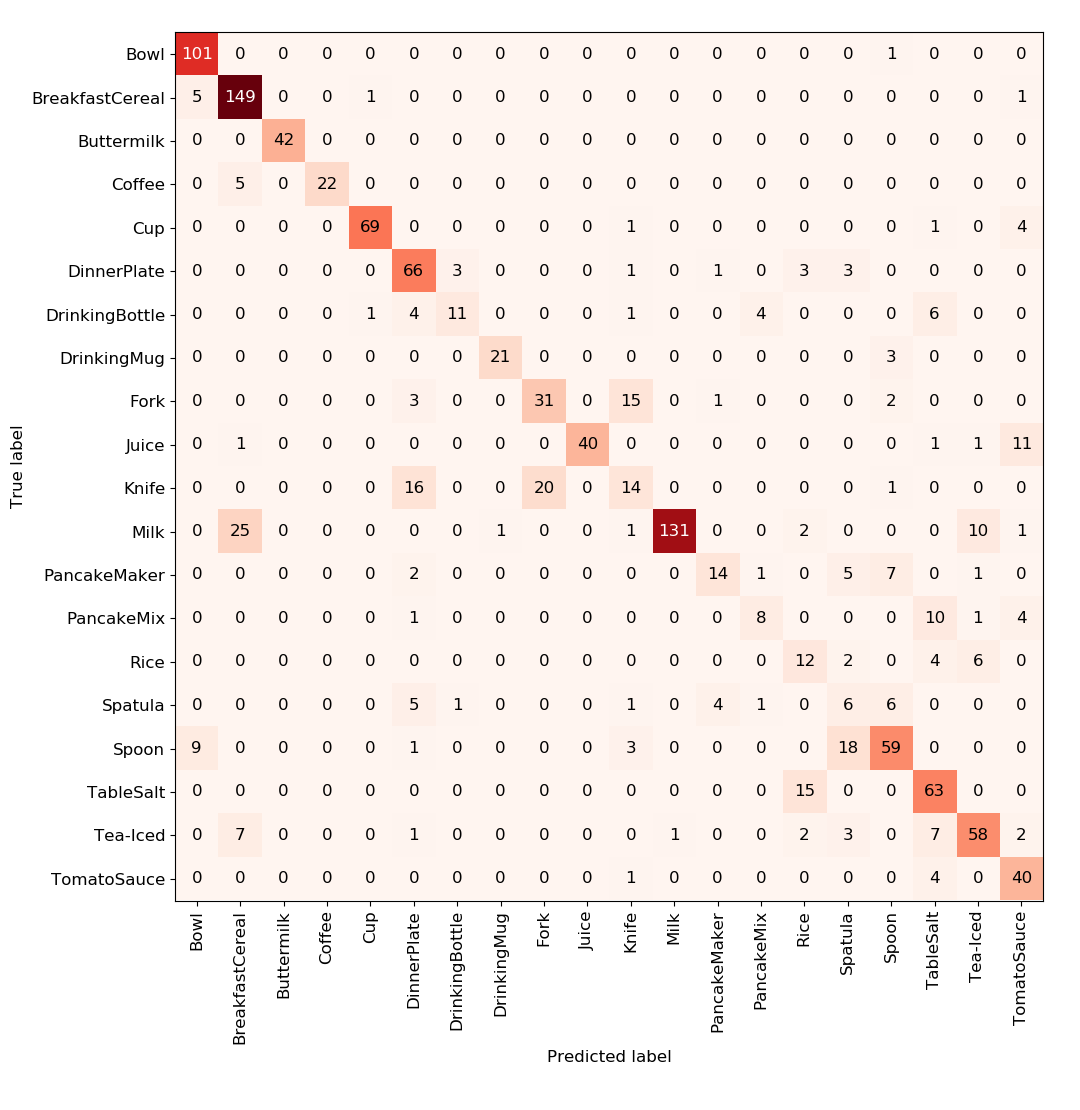
\includegraphics[scale=.315]{img/chapter6/UnrealRealGTCLass.png}
\caption[Konfusionsmatrix der Objektklassen Klassifikation mit Unreal-Trainingsset und realem Testset]{Die Konfusionsmatrix für die Klassifikation aller realen Bilder durch ein \gls{mln}, das mit allen Unreal-Bildern trainiert wurde. Als \gls{gt} wurden die Objektklassen verwendet.}
\label{fig:UnrealRealGTClass_confMatrix}
\end{figure}  

\section{Reale Bilder als Testdaten}

Im folgenden Experiment wird ein \gls{mln} mit den Unreal-Bildern trainiert und mit den realen Bildern getestet. Die Unreal-Bilder wurden wie zuvor von der in Kapitel \ref{sec:analysisengine} beschriebenen \gls{ae} annotiert. Die realen Bilder ebenfalls, allerdings ohne den \texttt{UnrealGTAnnotator} zu verwenden, da dieser nur für Bilder aus der \unreal geeignet ist und echte Bilder keine Asset-Namen zur Bestimmung der \gls{gt} aufweisen. Dementsprechend wurde die \gls{gt} manuell annotiert. Damit die Atome für den \texttt{GogglesAnnotator} in beiden Datensätzen übereinstimmen, wurde das Clustering mit den Annotationen aus beiden Datensätzen durchgeführt. Die Deklaration des \gls{mln} und Parameter beim Lernen und Anfragen sind unverändert gegenüber dem vorherigen Experiment. \par

\subsection{Objektklassen}

Bei der Klassifizierung der Objektklassen (Abbildung \ref{fig:UnrealRealGTClass_confMatrix}, Tabelle \ref{tab:UnrealRealGTClass_metrics}) ist die \gls{accuracy} für alle Klassen über 90\%, während auch die Werte für \gls{precision}, \gls{recall} und \gls{f1score} in den meisten Fällen mit über 70\% relativ hoch ausfallen. Ausnahmen bilden wie erwartet das Besteck, aber auch \textit{DrinkingBottle}, \textit{PancakeMix} und \textit{PancakeMaker} und der \textit{Rice}. Interessanterweise schneiden \textit{Spoons} und \textit{Forks} dabei deutlich besser ab als \textit{Knives}. Besonders schlecht schneidet auch der \textit{Spatula} ab, was auch schon bei den \glspl{klassifikator} aufgefallen war. Da die 10-fache Kreuzvalidierung, bei der nur Unreal-Bilder verwendet wurden, dieses Problem nicht zeigte, kann angenommen werden, dass das 3D-Modell keine gute Repräsentation des echten Objektes darstellt. Dass die Performance bei \textit{Rice} so stark abfällt, ist interessant, da die Erkennungsrate für andere texturierte Objekte (\textit{BreakfastCereal}, \textit{Milk}, \textit{TableSalt}, \textit{Tea-Iced}, \textit{TomatoSauce}) nicht so stark abfällt. Der wahrscheinlich wegen seiner Form von den \glspl{klassifikator} noch gut erkannte \textit{PancakeMix} scheint diesen Vorteil hier nicht ausspielen zu können, während das für \textit{Buttermilk} mit einer 100 prozentigen Klassifikationsrate nicht gilt. Für den \textit{PancakeMaker} scheint dasselbe zu gelten wie für den \textit{Spatula}, da auch er schon bei den \glspl{klassifikator} eine Problemquelle darstellte. 

\begin{table}
\centering
\small
\rowcolors{1}{}{lightgray}
\begin{tabularx}{\textwidth}{Xllll}
\textbf{Objekt}	& \textbf{\gls{accuracy}} & \textbf{\gls{precision}}	& \textbf{\gls{recall}}	& \textbf{\gls{f1score}} \\ \hline
Bowl & 0.98 & 0.88 & 0.99 & 0.93 \\  
BreakfastCereal & 0.96 & 0.8 & 0.96 & 0.87 \\  
Buttermilk & 1.0 & 1.0 & 1.0 & 1.0 \\  
Coffee & 0.99 & 1.0 & 0.81 & 0.9 \\  
Cup & 0.99 & 0.97 & 0.92 & 0.95 \\  
DinnerPlate & 0.96 & 0.67 & 0.86 & 0.75 \\  
DrinkingBottle & 0.98 & 0.73 & 0.41 & 0.52 \\  
DrinkingMug & 1.0 & 0.95 & 0.88 & 0.91 \\  
Fork & 0.96 & 0.61 & 0.6 & 0.6 \\  
Juice & 0.99 & 1.0 & 0.74 & 0.85 \\  
Knife & 0.94 & 0.37 & 0.27 & 0.31 \\  
Milk & 0.96 & 0.99 & 0.77 & 0.86 \\  
PancakeMaker & 0.98 & 0.7 & 0.47 & 0.56 \\  
PancakeMix & 0.98 & 0.57 & 0.33 & 0.42 \\  
Rice & 0.97 & 0.35 & 0.5 & 0.41 \\  
Spatula & 0.95 & 0.16 & 0.25 & 0.2 \\  
Spoon & 0.95 & 0.75 & 0.66 & 0.7 \\  
TableSalt & 0.95 & 0.66 & 0.81 & 0.72 \\  
Tea-Iced & 0.96 & 0.75 & 0.72 & 0.73 \\  
TomatoSauce & 0.97 & 0.63 & 0.89 & 0.74 \\   \hline
\textbf{Gesamt}		&	\textbf{0.76}   &	\textbf{0.78}  & \textbf{0.76}     &  \textbf{0.76}    \\
\end{tabularx}
\caption[Objektklassen-spezifische Kenngrößen der Klassifikation mit Unreal-Trainingsset und realem Testset]{Kenngrößen für die einzelnen Objekte der Klassifikation der realen Bilder durch ein \gls{mln}, das mit allen Unreal-Bildern trainiert wurde. Als \gls{gt} wurden die Objektklassen verwendet.}
\label{tab:UnrealRealGTClass_metrics}
\end{table}

\subsection{Instanznamen}

Die Ergebnisse für die Klassifikation mit den Instanznamen als \gls{gt} sind in Abbildung \ref{fig:UnrealRealGTInstance_confMatrix} und Tabelle \ref{tab:UnrealRealGTInstance_metrics} zu finden. Im Gegensatz zur 10-fachen Kreuzvalidierung des gesamten Unreal-Bilder Satzes steigert sich die Erkennungsrate gegenüber den Objektklassen nicht leicht, sondern verschlechtert sich. Als Probleme fallen mal wieder der \textit{SlottedSpatula} und der \textit{LargeGreySpoon} ins Auge, die wieder häufig verwechselt werden. Am schlechtesten schneidet die \textit{WhiteCeramicIkeaBowl} ab, die meistens für die \textit{BluePlasticBowl} gehalten wird, welche auch häufiger falsch klassifiziert wurde. Ähnliche Ergebnisse der beiden Schüsseln waren auch bei den \glspl{klassifikator} zu beobachten. Das kleine Besteck schneidet wie üblich nicht so gut ab. Während \textit{Spoons} allerdings in fast allen \gls{mln} Klassifikationen das am besten erkannte Besteck sind, bildeten sie bei den \glspl{klassifikator} noch das Schlusslicht. Ansonsten gibt es die zuvor schon erwähnten Ungenauigkeiten bei ähnlich farbigen und/oder texturierten Objekten aus \textit{TableSalt}, \textit{Milk}, \textit{Tea-Iced}, \textit{BreakfastCereal} und \textit{PancakeMix}. \par

\begin{figure}
\centering
	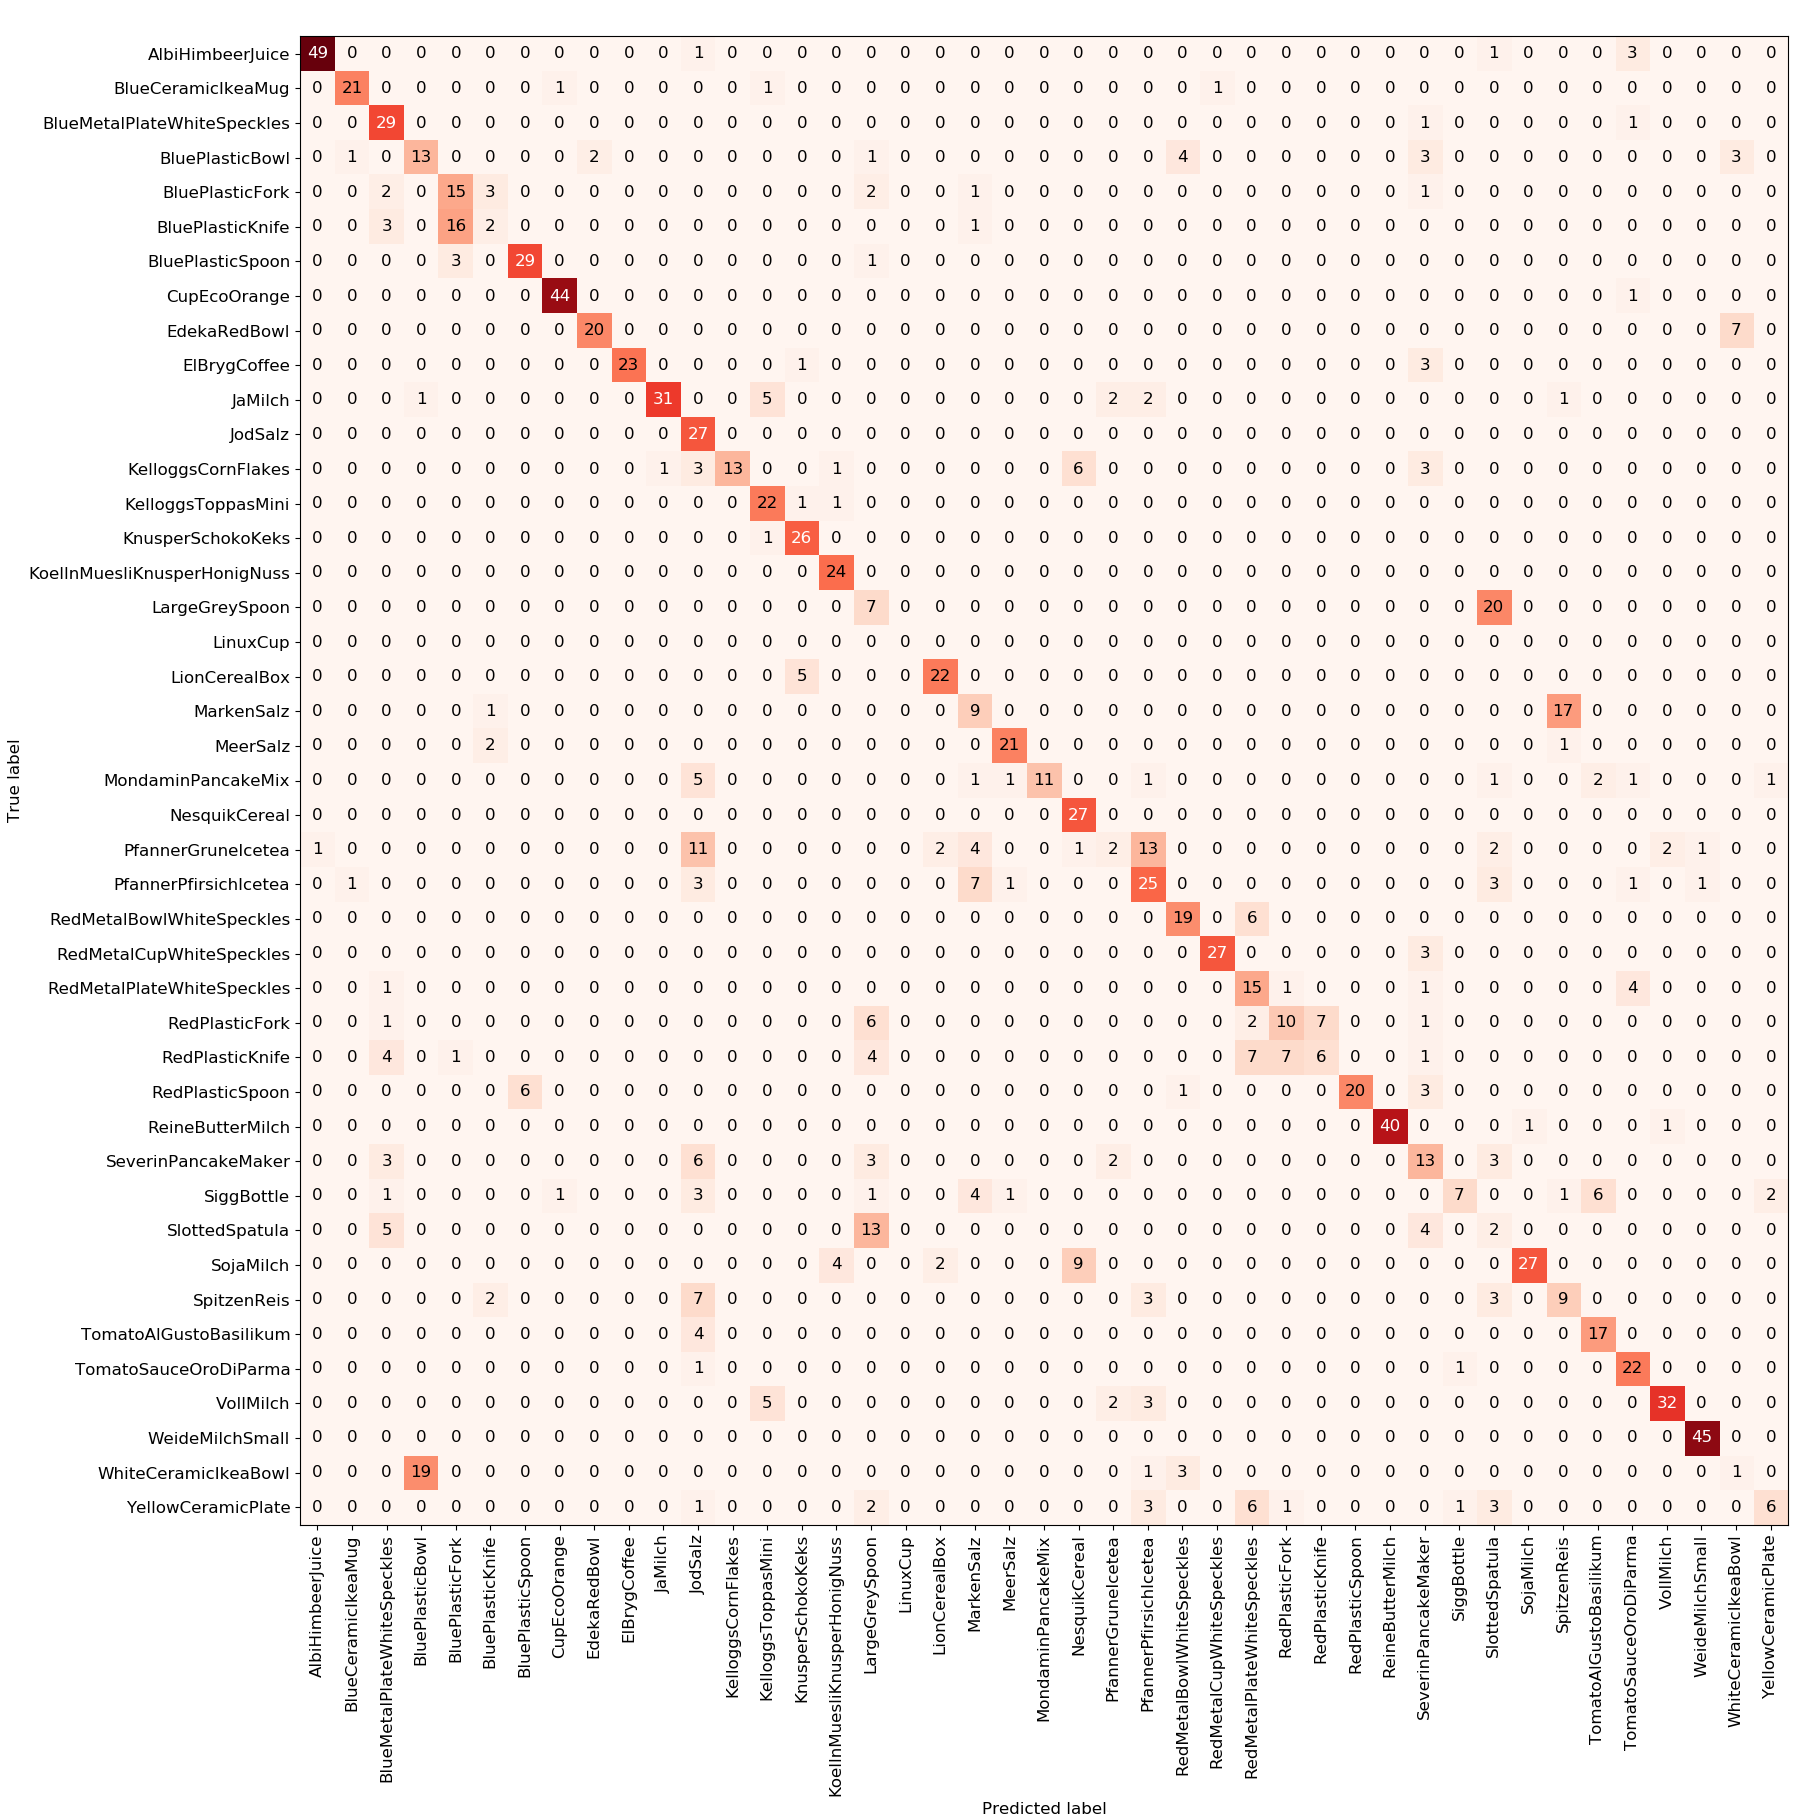
\includegraphics[scale=.292]{img/chapter6/UnrealRealGTInstance.png}
\caption[Konfusionsmatrix der Objektinstanzen Klassifikation mit Unreal-Trainingsset und realem Testset]{Die Konfusionsmatrix für die Klassifikation aller realen Bilder durch ein \gls{mln}, das mit allen Unreal-Bildern trainiert wurde. Als \gls{gt} wurden die Objektinstanzen verwendet.}
\label{fig:UnrealRealGTInstance_confMatrix}
\end{figure} 

\begin{table}
\centering
\small
\rowcolors{1}{}{lightgray}
\begin{tabularx}{\textwidth}{Xllll}
\textbf{Objekt}	& \textbf{\gls{accuracy}} & \textbf{\gls{precision}}	& \textbf{\gls{recall}}	& \textbf{\gls{f1score}} \\ \hline
AlbiHimbeerJuice & 0.99 & 0.98 & 0.91 & 0.94 \\  
BlueCeramicIkeaMug & 0.99 & 0.91 & 0.88 & 0.89 \\  
BlueMetalPlateWhiteSpeckles & 0.97 & 0.59 & 0.94 & 0.72 \\  
BluePlasticBowl & 0.96 & 0.39 & 0.48 & 0.43 \\  
BluePlasticFork & 0.97 & 0.43 & 0.63 & 0.51 \\  
BluePlasticKnife & 0.97 & 0.2 & 0.09 & 0.13 \\  
BluePlasticSpoon & 0.99 & 0.83 & 0.88 & 0.85 \\  
CupEcoOrange & 1.0 & 0.96 & 0.98 & 0.97 \\  
EdekaRedBowl & 0.99 & 0.91 & 0.74 & 0.82 \\  
ElBrygCoffee & 1.0 & 1.0 & 0.85 & 0.92 \\  
JaMilch & 0.99 & 0.97 & 0.74 & 0.84 \\  
JodSalz & 0.95 & 0.38 & 1.0 & 0.55 \\  
KelloggsCornFlakes & 0.98 & 1.0 & 0.48 & 0.65 \\  
KelloggsToppasMini & 0.98 & 0.65 & 0.92 & 0.76 \\  
KnusperSchokoKeks & 0.99 & 0.79 & 0.96 & 0.87 \\  
KoellnMuesliKnusperHonigNuss & 0.99 & 0.8 & 1.0 & 0.89 \\  
LargeGreySpoon & 0.94 & 0.17 & 0.26 & 0.21 \\  
LinuxCup & 1.0 & 0.0 & 0.0 & 0.0 \\  
LionCerealBox & 0.99 & 0.85 & 0.81 & 0.83 \\  
MarkenSalz & 0.96 & 0.33 & 0.33 & 0.33 \\  
MeerSalz & 0.99 & 0.88 & 0.88 & 0.88 \\  
MondaminPancakeMix & 0.98 & 1.0 & 0.46 & 0.63 \\  
NesquikCereal & 0.98 & 0.63 & 1.0 & 0.77 \\  
PfannerGruneIcetea & 0.95 & 0.25 & 0.05 & 0.09 \\  
PfannerPfirsichIcetea & 0.95 & 0.49 & 0.6 & 0.54 \\  
RedMetalBowlWhiteSpeckles & 0.98 & 0.7 & 0.76 & 0.73 \\  
RedMetalCupWhiteSpeckles & 1.0 & 0.96 & 0.9 & 0.93 \\  
RedMetalPlateWhiteSpeckles & 0.97 & 0.42 & 0.68 & 0.52 \\  
RedPlasticFork & 0.97 & 0.53 & 0.37 & 0.43 \\  
RedPlasticKnife & 0.96 & 0.46 & 0.2 & 0.28 \\  
RedPlasticSpoon & 0.99 & 1.0 & 0.67 & 0.8 \\  
ReineButterMilch & 1.0 & 1.0 & 0.95 & 0.98 \\  
SeverinPancakeMaker & 0.95 & 0.35 & 0.43 & 0.39 \\  
SiggBottle & 0.97 & 0.78 & 0.26 & 0.39 \\  
SlottedSpatula & 0.93 & 0.05 & 0.08 & 0.06 \\  
SojaMilch & 0.98 & 0.96 & 0.64 & 0.77 \\  
SpitzenReis & 0.96 & 0.31 & 0.38 & 0.34 \\  
TomatoAlGustoBasilikum & 0.99 & 0.68 & 0.81 & 0.74 \\  
TomatoSauceOroDiParma & 0.98 & 0.67 & 0.92 & 0.77 \\  
VollMilch & 0.98 & 0.91 & 0.76 & 0.83 \\  
WeideMilchSmall & 1.0 & 0.96 & 1.0 & 0.98 \\  
WhiteCeramicIkeaBowl & 0.96 & 0.09 & 0.04 & 0.06 \\  
YellowCeramicPlate & 0.98 & 0.67 & 0.26 & 0.38 \\     \hline
\textbf{Gesamt}		&	\textbf{0.66}   &	\textbf{0.69}  & \textbf{0.66}     &  \textbf{0.65}    \\
\end{tabularx}
\caption[Objektinstanzen-spezifische Kenngrößen der Klassifikation mit Unreal-Trainingsset und realem Testset]{Kenngrößen für die einzelnen Objekte der Klassifikation der realen Bilder durch ein \gls{mln}, das mit allen Unreal-Bildern trainiert wurde. Als \gls{gt} wurden die Objektinstanzen verwendet.}
\label{tab:UnrealRealGTInstance_metrics}
\end{table} 


\begin{table}
\centering
\rowcolors{1}{}{lightgray}
\begin{tabularx}{\textwidth}{Xlllllll}
\textbf{Klassifi.}	&\textbf{Training}&\textbf{Test}&	\textbf{\gls{gt}}	& \textbf{\gls{accuracy}} & \textbf{\gls{precision}}	& \textbf{\gls{recall}}	& \textbf{\gls{f1score}} \\ \hline
RF	&-	&U	&Klasse		&0.6	&0.67	&0.6	&0.57	\\
SVM	&-	&U	&Klasse		&0.62	&0.7	&0.62	&0.57	\\
RF	&-	&U	&Instanz	&0.6	&0.62	&0.6	&0.58	\\
SVM	&-	&U	&Instanz	&0.66	&0.72	&0.66	&0.62	\\ \hline
MLN	&U	&U	&Klasse		&0.95	&0.95	&0.95	&0.95	\\
MLN	&U	&U	&Instanz	&0.96	&0.96	&0.96	&0.96	\\ \hline
MLN	&U	&R	&Klasse		&0.76	&0.78	&0.76	&0.76	\\
MLN	&U	&R	&Instanz	&0.66	&0.69	&0.66	&0.65	\\ \hline
MLN	&U/R&R	&Klasse		&0.9	&0.91	&0.9	&0.9	\\
MLN	&U/R&R	&Instanz	&0.88	&0.88	&0.88	&0.88	\\ \hline \hline
MLN &R	&R	&Klasse 	&0.69	&0.69	&0.69	&0.69 \\ 
\end{tabularx}
\caption[Übersicht der Kenngrößen der einzelnen Experimente]{Die Tabelle enthält die einzelnen Mittelwerte der Kenngrößen der Klassifikationen aus den jeweiligen Experimenten. Die erste Spalte beschreibt den verwendeten Klassifikator bzw. ob ein \gls{mln} verwendet wurde und richtet sich nach der Reihenfolge der Experimente in dieser Arbeit. Die Spalten Training und Test beschreiben die jeweils verwendeten Datensätze: U für Unreal-Bilder, R für reale Bilder. Die letzte Zeile enthält die Ergebnisse der Klassifikation aus \cite{pr2looking}. Dabei wurde ein \gls{mln} mit realen Bildern trainiert und getestet. Die verwendeten Bilder und Klassen sind allerdings andere als in dieser Arbeit.}
\label{tab:classification_all}
\end{table}

%\begin{figure}
%\centering
%	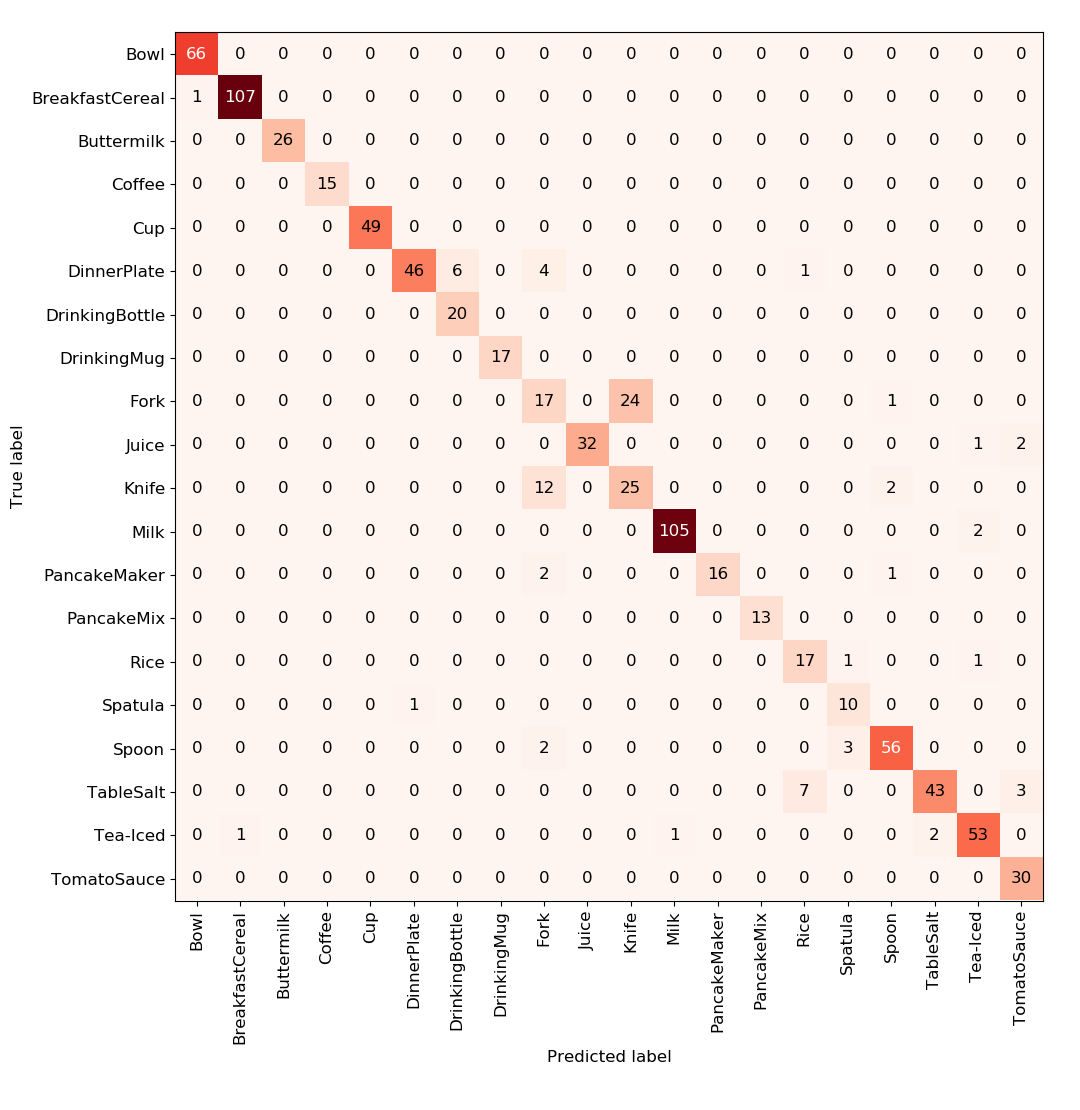
\includegraphics[scale=.315]{img/chapter6/UnrealRealMixedGTClass.png}
%\caption[Konfusionsmatrix der Objektklassen Klassifikation mit gemischtem Trainingsset und realem Testset]{Die Konfusionsmatrix für die \gls{mln}-Klassifikation der Klassen. Trainingsset sind alle Unreal-Bildern und ein drittel der realen Bilder, die restlichen.}
%\label{fig:UnrealRealMixedGTClass_confMatrix}
%\end{figure} 

\section{Ein gemischtes Trainigsset}
\label{unrealrealmixed}

Im letzten Experiment wurde ein Teil der realen Bilder zusätzlich zu den Unreal-Bildern zum Trainieren verwendet. Dazu wurde zufällig ein Drittel der realen Bilder ausgewählt, womit insgesamt mit 684 Bildern trainiert wurde. Die restlichen 228 realen Bilder wurden wieder als Testdaten verwendet. \par

Die Konfusionsmatrizen sind in Abbildung \ref{fig:UnrealRealMixed_confMatrices} zu finden. Die Kenngrößen für die gesamte Klassifikation finden sich in Tabelle \ref{tab:classification_all}. Für beide \gls{gt}s hat sich die Performance gegenüber dem vorherigen Experiment gesteigert, sodass beide bei allen Werten im Bereich um die 90\% liegen. Die meisten großen Fehlerquellen wurden durch das gemischte Trainingsset eliminiert. Nur die \textit{Knives} und \textit{Forks} bleiben wieder deutlich hinter dem Rest zurück. Allerdings haben sich die Werte für die Messer deutlich verbessert und liegen nun im Bereich der Gabeln und nicht wie zuvor deutlich darunter.  \par 

\begin{figure}
\centering
	\begin{subfigure}[b]{1\textwidth}
	\centering
	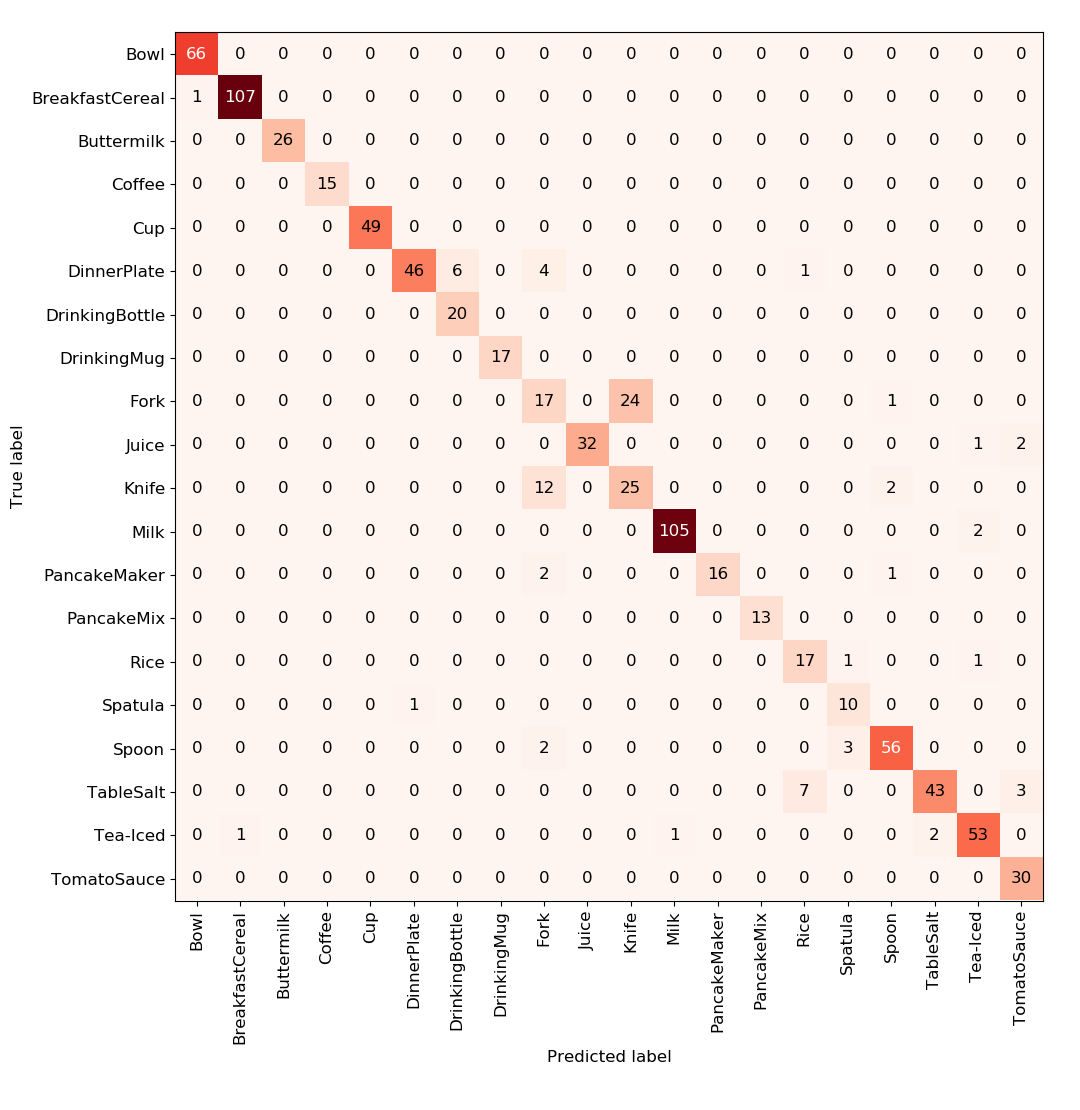
\includegraphics[scale=.29]{img/chapter6/UnrealRealMixedGTClass.png}
	\end{subfigure}
	\begin{subfigure}[b]{1\textwidth}
	\centering
	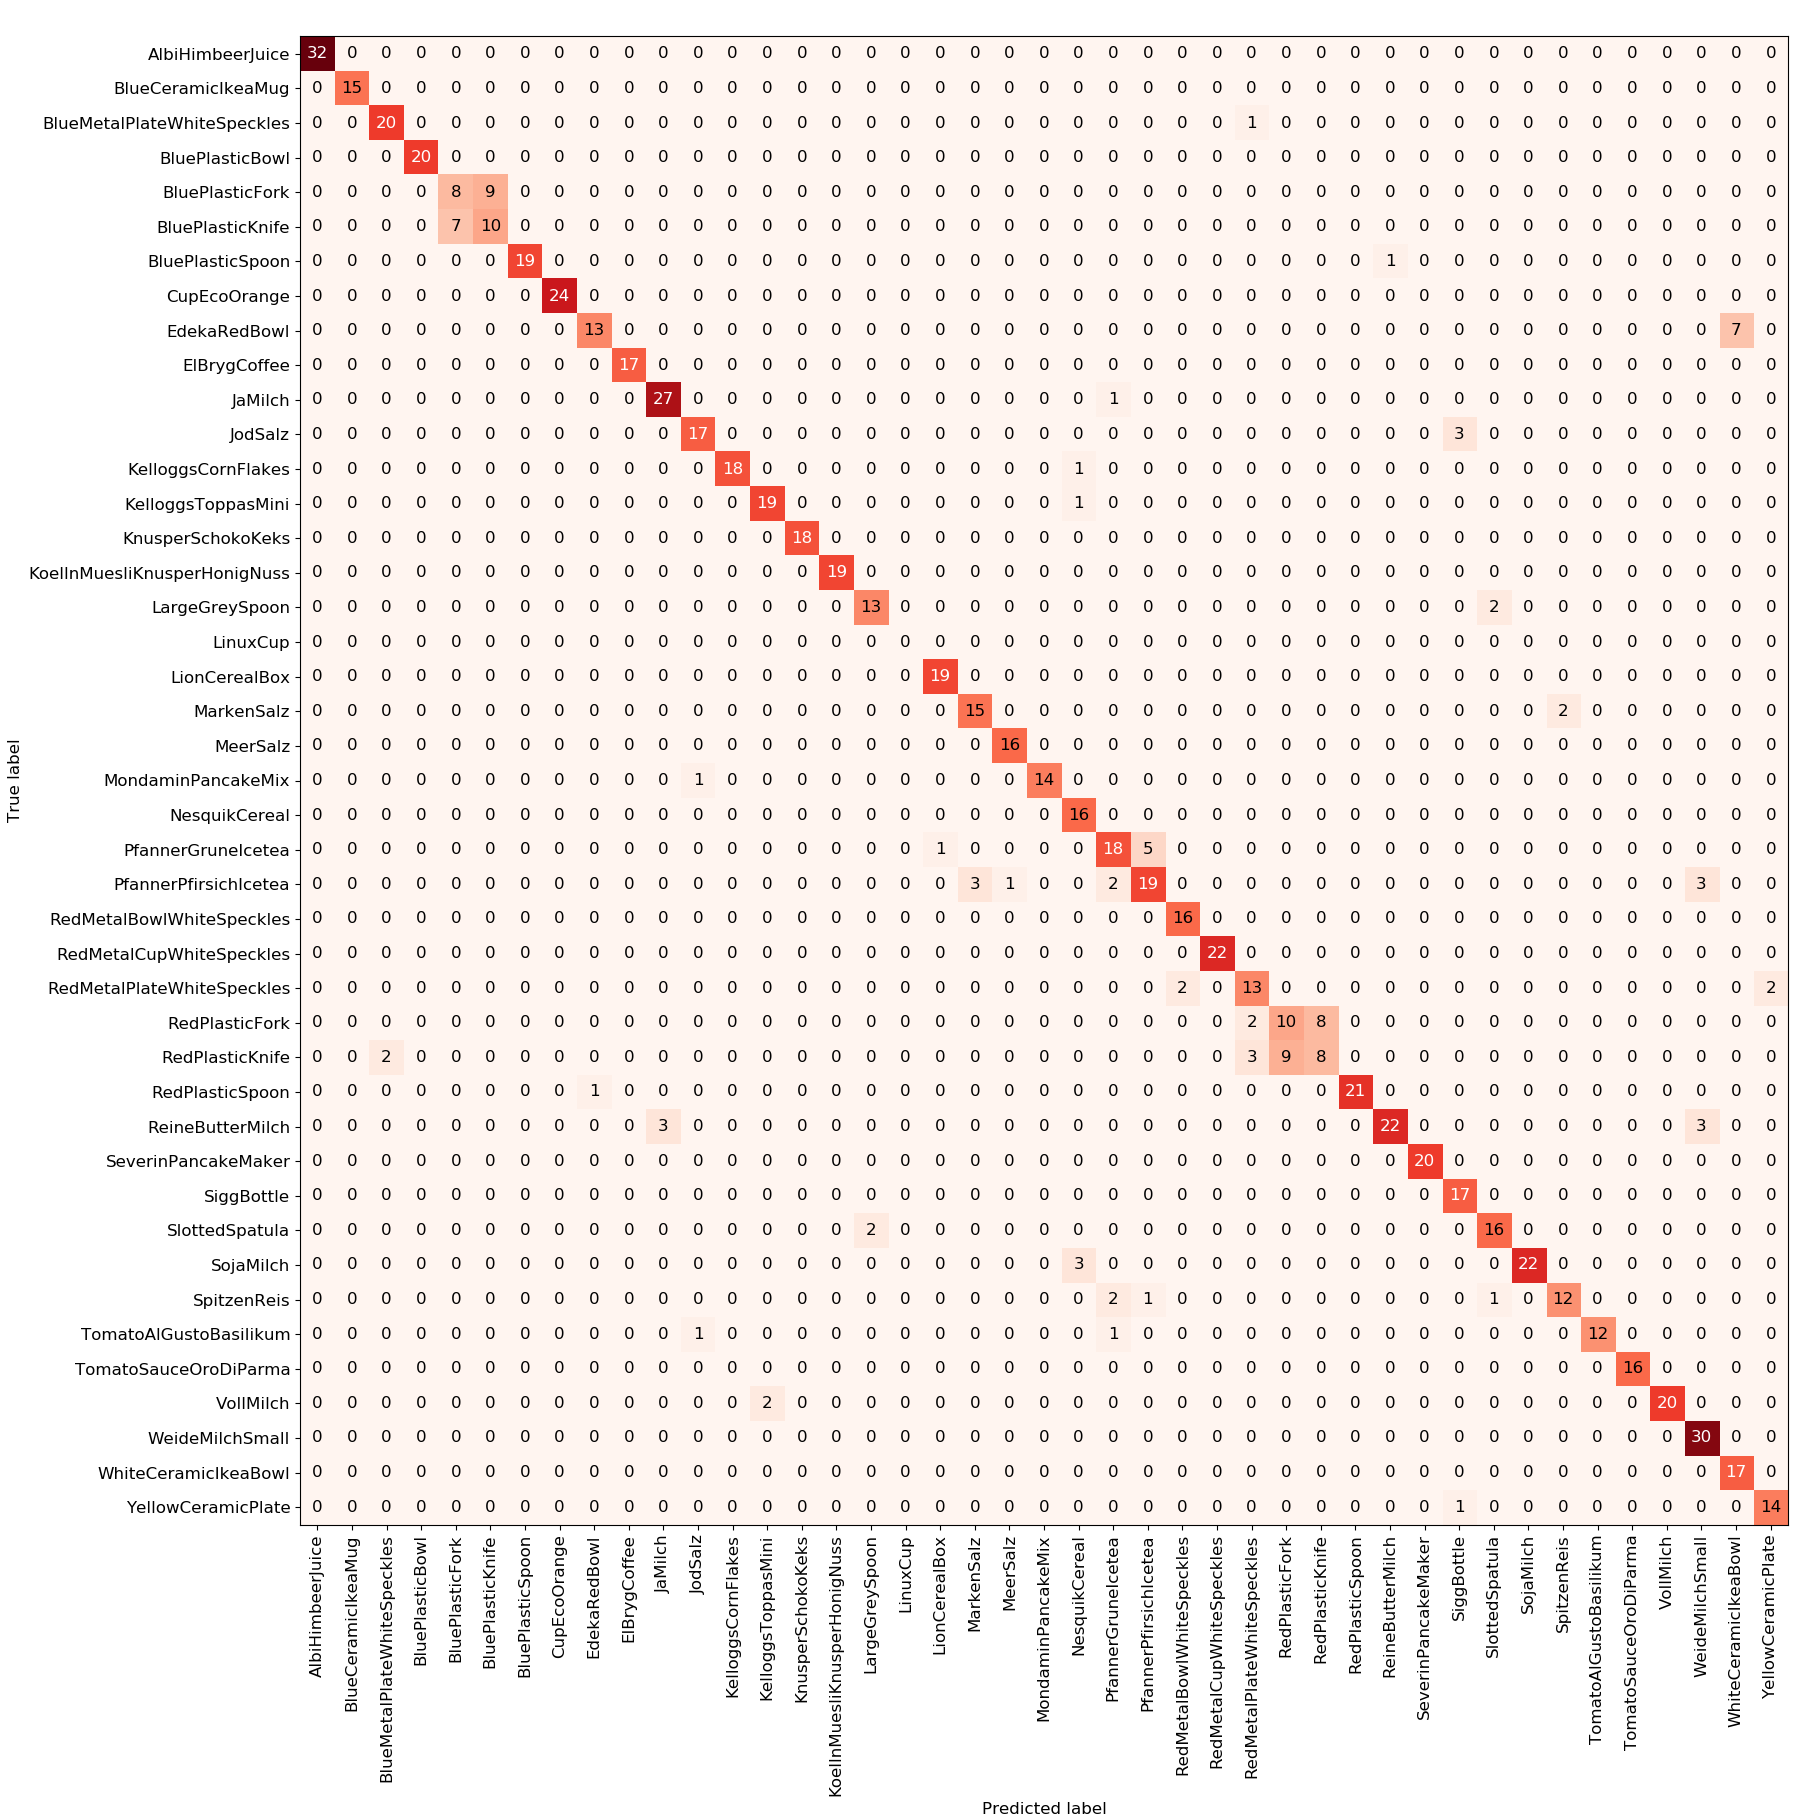
\includegraphics[scale=.29]{img/chapter6/UnrealRealMixedGTInstance.png}
	\end{subfigure}
\caption[Die Konfusionsmatrizen der Klassifikation mit gemischtem Trainingsset und realem Testset]{Die Konfusionsmatrizen für die \gls{mln}-Klassifikation mit gemischtem Trainingsset. Es besteht aus allen Unreal-Bildern und einem drittel der realen Bilder, die Restlichen bilden das Testset.}
\label{fig:UnrealRealMixed_confMatrices}
\end{figure}

%\begin{figure}
%\centering
%	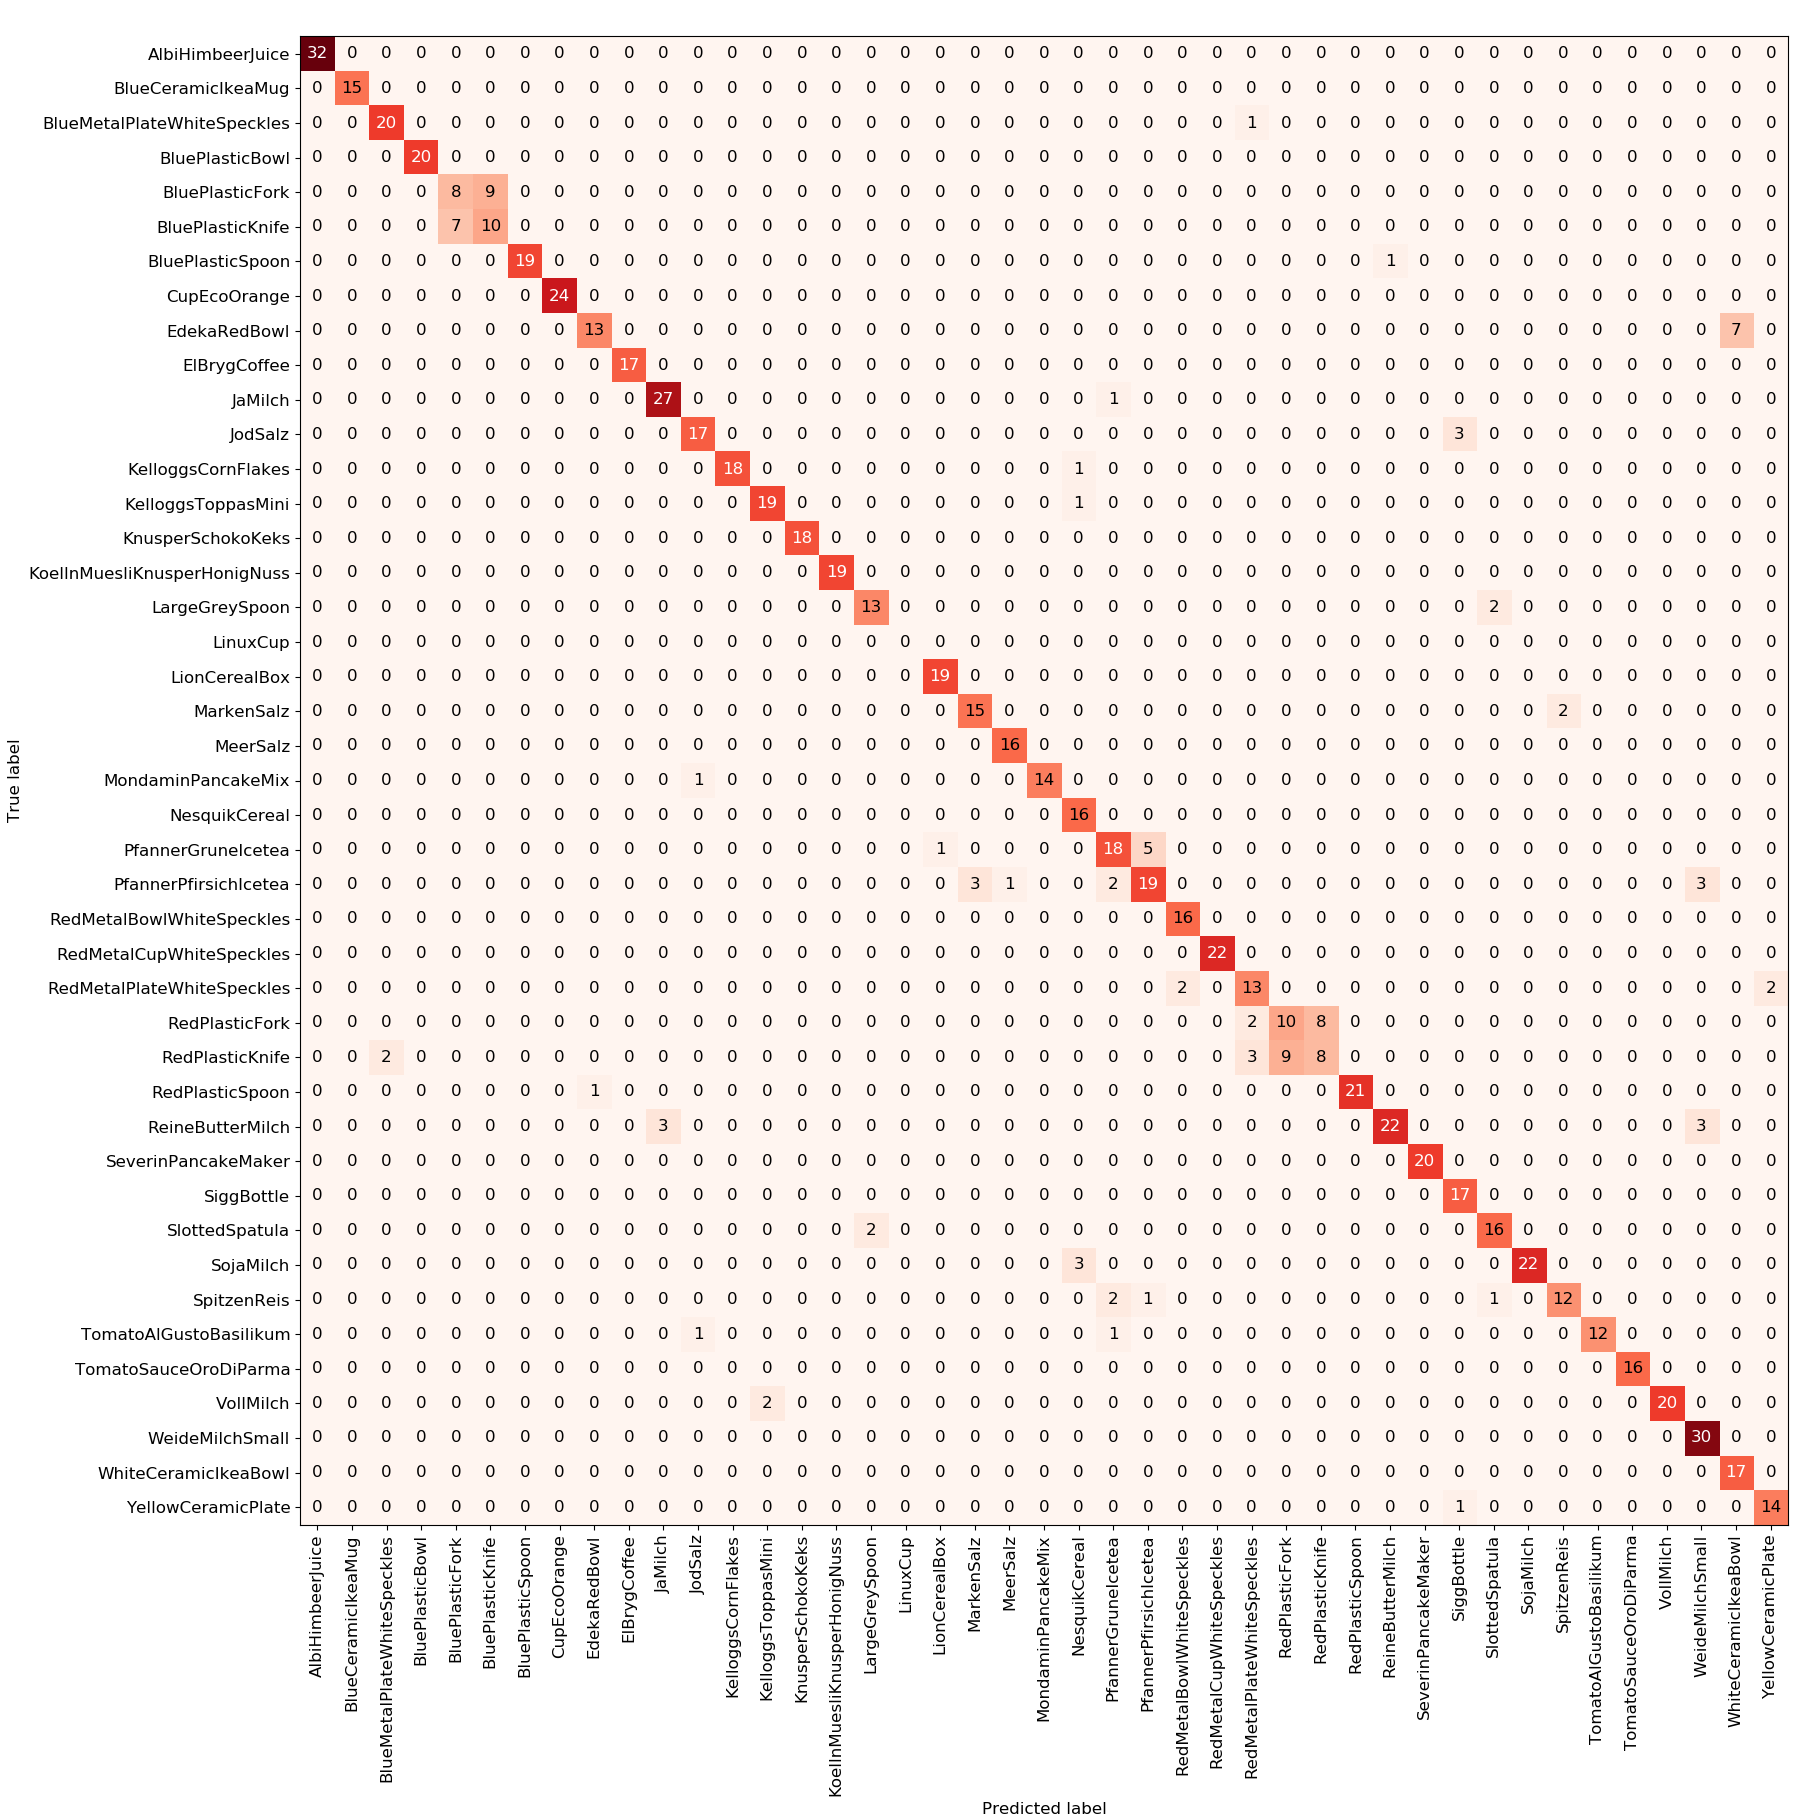
\includegraphics[scale=.292]{img/chapter6/UnrealRealMixedGTInstance.png}
%\caption[Konfusionsmatrix der Objektinstanzen Klassifikation mit gemischtem Trainingsset und realem Testset]{Die Konfusionsmatrix für die \gls{mln}-Klassifikation der Instanzen. Trainingsset sind alle Unreal-Bildern und ein drittel der realen Bilder, die restlichen bilden das Testset.}
%\label{fig:UnrealRealMixedGTInstance_confMatrix}
%\end{figure} 

%\begin{table}
%\centering
%\rowcolors{1}{}{lightgray}
%\begin{tabularx}{\textwidth}{Xllll}
%\textbf{Objekt}	& \textbf{\gls{accuracy}} & \textbf{\gls{precision}}	& \textbf{\gls{recall}}	& \textbf{\gls{f1score}} \\ \hline
%Bowl & 1.0 & 0.99 & 1.0 & 0.99 \\  
%BreakfastCereal & 1.0 & 0.99 & 0.99 & 0.99 \\  
%Buttermilk & 1.0 & 1.0 & 1.0 & 1.0 \\  
%Coffee & 1.0 & 1.0 & 1.0 & 1.0 \\  
%Cup & 1.0 & 1.0 & 1.0 & 1.0 \\  
%DinnerPlate & 0.98 & 0.98 & 0.81 & 0.88 \\  
%DrinkingBottle & 0.99 & 0.77 & 1.0 & 0.87 \\  
%DrinkingMug & 1.0 & 1.0 & 1.0 & 1.0 \\  
%Fork & 0.94 & 0.46 & 0.4 & 0.43 \\  
%Juice & 1.0 & 1.0 & 0.91 & 0.96 \\  
%Knife & 0.95 & 0.51 & 0.64 & 0.57 \\  
%Milk & 1.0 & 0.99 & 0.98 & 0.99 \\  
%PancakeMaker & 1.0 & 1.0 & 0.84 & 0.91 \\  
%PancakeMix & 1.0 & 1.0 & 1.0 & 1.0 \\  
%Rice & 0.99 & 0.68 & 0.89 & 0.77 \\  
%Spatula & 0.99 & 0.71 & 0.91 & 0.8 \\  
%Spoon & 0.99 & 0.93 & 0.92 & 0.93 \\  
%TableSalt & 0.98 & 0.96 & 0.81 & 0.88 \\  
%Tea-Iced & 0.99 & 0.93 & 0.93 & 0.93 \\  
%TomatoSauce & 0.99 & 0.86 & 1.0 & 0.92 \\  \hline
%\textbf{Gesamt}	&	\textbf{0.9}   &	\textbf{0.91}  & \textbf{0.9}   & \textbf{0.91} \\
%\end{tabularx}
%\caption[Objektklassen-spezifische Kenngrößen der Klassifikation mit gemischtem Trainingsset und realem Testset]{Kenngrößen für die einzelnen Objekte der Klassifikation durch ein \gls{mln}, das mit allen Unreal-Bildern und einem drittel der realen Bilder trainiert wurde. Getestet wurde mit den restlichen realen Bildern. Als \gls{gt} wurden die Objektklassen verwendet.}
%\label{tab:UnrealRealMixedGTClass_metrics}
%\end{table}

%\begin{table}
%\centering
%\small
%\rowcolors{1}{}{lightgray}
%\begin{tabularx}{\textwidth}{Xllll}
%\textbf{Objekt}	& \textbf{\gls{accuracy}} & \textbf{\gls{precision}}	& \textbf{\gls{recall}}	& \textbf{\gls{f1score}} \\ \hline
%AlbiHimbeerJuice & 1.0 & 1.0 & 1.0 & 1.0 \\  
%BlueCeramicIkeaMug & 1.0 & 1.0 & 1.0 & 1.0 \\  
%BlueMetalPlateWhiteSpeckles & 1.0 & 0.91 & 0.95 & 0.93 \\  
%BluePlasticBowl & 1.0 & 1.0 & 1.0 & 1.0 \\  
%BluePlasticFork & 0.98 & 0.53 & 0.47 & 0.5 \\  
%BluePlasticKnife & 0.98 & 0.53 & 0.59 & 0.56 \\  
%BluePlasticSpoon & 1.0 & 1.0 & 0.95 & 0.97 \\  
%CupEcoOrange & 1.0 & 1.0 & 1.0 & 1.0 \\  
%EdekaRedBowl & 0.99 & 0.93 & 0.65 & 0.76 \\  
%ElBrygCoffee & 1.0 & 1.0 & 1.0 & 1.0 \\  
%JaMilch & 0.99 & 0.9 & 0.96 & 0.93 \\  
%JodSalz & 0.99 & 0.89 & 0.85 & 0.87 \\  
%KelloggsCornFlakes & 1.0 & 1.0 & 0.95 & 0.97 \\  
%KelloggsToppasMini & 1.0 & 0.9 & 0.95 & 0.93 \\  
%KnusperSchokoKeks & 1.0 & 1.0 & 1.0 & 1.0 \\  
%KoellnMuesliKnusperHonigNuss & 1.0 & 1.0 & 1.0 & 1.0 \\  
%LargeGreySpoon & 0.99 & 0.87 & 0.87 & 0.87 \\  
%LinuxCup & 1.0 & 0.0 & 0.0 & 0.0 \\  
%LionCerealBox & 1.0 & 0.95 & 1.0 & 0.97 \\  
%MarkenSalz & 0.99 & 0.83 & 0.88 & 0.86 \\  
%MeerSalz & 1.0 & 0.94 & 1.0 & 0.97 \\  
%MondaminPancakeMix & 1.0 & 1.0 & 0.93 & 0.97 \\  
%NesquikCereal & 0.99 & 0.76 & 1.0 & 0.86 \\  
%PfannerGruneIcetea & 0.98 & 0.75 & 0.75 & 0.75 \\  
%PfannerPfirsichIcetea & 0.98 & 0.76 & 0.68 & 0.72 \\  
%RedMetalBowlWhiteSpeckles & 1.0 & 0.89 & 1.0 & 0.94 \\  
%RedMetalCupWhiteSpeckles & 1.0 & 1.0 & 1.0 & 1.0 \\  
%RedMetalPlateWhiteSpeckles & 0.99 & 0.68 & 0.76 & 0.72 \\  
%RedPlasticFork & 0.97 & 0.53 & 0.5 & 0.51 \\  
%RedPlasticKnife & 0.97 & 0.5 & 0.36 & 0.42 \\  
%RedPlasticSpoon & 1.0 & 1.0 & 0.95 & 0.98 \\  
%ReineButterMilch & 0.99 & 0.96 & 0.79 & 0.86 \\  
%SeverinPancakeMaker & 1.0 & 1.0 & 1.0 & 1.0 \\  
%SiggBottle & 0.99 & 0.81 & 1.0 & 0.89 \\  
%SlottedSpatula & 0.99 & 0.84 & 0.89 & 0.86 \\  
%SojaMilch & 1.0 & 1.0 & 0.88 & 0.94 \\  
%SpitzenReis & 0.99 & 0.86 & 0.75 & 0.8 \\  
%TomatoAlGustoBasilikum & 1.0 & 1.0 & 0.86 & 0.92 \\  
%TomatoSauceOroDiParma & 1.0 & 1.0 & 1.0 & 1.0 \\  
%VollMilch & 1.0 & 1.0 & 0.91 & 0.95 \\  
%WeideMilchSmall & 0.99 & 0.83 & 1.0 & 0.91 \\  
%WhiteCeramicIkeaBowl & 0.99 & 0.71 & 1.0 & 0.83 \\  
%YellowCeramicPlate & 1.0 & 0.88 & 0.93 & 0.9 \\   \hline
%\textbf{Gesamt}	& \textbf{0.88}   &	\textbf{0.88}  & \textbf{0.88} & \textbf{0.88}   \\
%\end{tabularx}
%\caption[Objektinstanzen-spezifische Kenngrößen der Klassifikation mit gemischtem Trainingsset und realem Testset]{Kenngrößen für die einzelnen Objekte der Klassifikation durch ein \gls{mln}, das mit allen Unreal-Bildern und einem drittel der realen Bilder trainiert wurde. Getestet wurde mit den restlichen realen Bildern. Als \gls{gt} wurden die Objektinstanzen verwendet.}
%\label{tab:UnrealRealMixedGTInstance_metrics}
%\end{table}
